\documentclass[12pt,A4paper,]{article}
\usepackage{lmodern}
\usepackage{amssymb,amsmath}
\usepackage{ifxetex,ifluatex}
\usepackage{fixltx2e} % provides \textsubscript
\ifnum 0\ifxetex 1\fi\ifluatex 1\fi=0 % if pdftex
  \usepackage[T1]{fontenc}
  \usepackage[utf8]{inputenc}
\else % if luatex or xelatex
  \ifxetex
    \usepackage{mathspec}
  \else
    \usepackage{fontspec}
  \fi
  \defaultfontfeatures{Ligatures=TeX,Scale=MatchLowercase}
    \setmainfont[]{PT Serif}
    \setsansfont[]{PT Sans}
    \setmonofont[Mapping=tex-ansi]{PT Mono}
\fi
% use upquote if available, for straight quotes in verbatim environments
\IfFileExists{upquote.sty}{\usepackage{upquote}}{}
% use microtype if available
\IfFileExists{microtype.sty}{%
\usepackage{microtype}
\UseMicrotypeSet[protrusion]{basicmath} % disable protrusion for tt fonts
}{}
\usepackage[margin=1in]{geometry}
\usepackage{hyperref}
\hypersetup{unicode=true,
            pdftitle={Determining the impact of wind and wave action on temperature along the South Africa coastline.},
            pdfauthor={Amieroh Abrahams},
            pdfborder={0 0 0},
            breaklinks=true}
\urlstyle{same}  % don't use monospace font for urls
\usepackage{color}
\usepackage{fancyvrb}
\newcommand{\VerbBar}{|}
\newcommand{\VERB}{\Verb[commandchars=\\\{\}]}
\DefineVerbatimEnvironment{Highlighting}{Verbatim}{commandchars=\\\{\}}
% Add ',fontsize=\small' for more characters per line
\usepackage{framed}
\definecolor{shadecolor}{RGB}{248,248,248}
\newenvironment{Shaded}{\begin{snugshade}}{\end{snugshade}}
\newcommand{\KeywordTok}[1]{\textcolor[rgb]{0.13,0.29,0.53}{\textbf{#1}}}
\newcommand{\DataTypeTok}[1]{\textcolor[rgb]{0.13,0.29,0.53}{#1}}
\newcommand{\DecValTok}[1]{\textcolor[rgb]{0.00,0.00,0.81}{#1}}
\newcommand{\BaseNTok}[1]{\textcolor[rgb]{0.00,0.00,0.81}{#1}}
\newcommand{\FloatTok}[1]{\textcolor[rgb]{0.00,0.00,0.81}{#1}}
\newcommand{\ConstantTok}[1]{\textcolor[rgb]{0.00,0.00,0.00}{#1}}
\newcommand{\CharTok}[1]{\textcolor[rgb]{0.31,0.60,0.02}{#1}}
\newcommand{\SpecialCharTok}[1]{\textcolor[rgb]{0.00,0.00,0.00}{#1}}
\newcommand{\StringTok}[1]{\textcolor[rgb]{0.31,0.60,0.02}{#1}}
\newcommand{\VerbatimStringTok}[1]{\textcolor[rgb]{0.31,0.60,0.02}{#1}}
\newcommand{\SpecialStringTok}[1]{\textcolor[rgb]{0.31,0.60,0.02}{#1}}
\newcommand{\ImportTok}[1]{#1}
\newcommand{\CommentTok}[1]{\textcolor[rgb]{0.56,0.35,0.01}{\textit{#1}}}
\newcommand{\DocumentationTok}[1]{\textcolor[rgb]{0.56,0.35,0.01}{\textbf{\textit{#1}}}}
\newcommand{\AnnotationTok}[1]{\textcolor[rgb]{0.56,0.35,0.01}{\textbf{\textit{#1}}}}
\newcommand{\CommentVarTok}[1]{\textcolor[rgb]{0.56,0.35,0.01}{\textbf{\textit{#1}}}}
\newcommand{\OtherTok}[1]{\textcolor[rgb]{0.56,0.35,0.01}{#1}}
\newcommand{\FunctionTok}[1]{\textcolor[rgb]{0.00,0.00,0.00}{#1}}
\newcommand{\VariableTok}[1]{\textcolor[rgb]{0.00,0.00,0.00}{#1}}
\newcommand{\ControlFlowTok}[1]{\textcolor[rgb]{0.13,0.29,0.53}{\textbf{#1}}}
\newcommand{\OperatorTok}[1]{\textcolor[rgb]{0.81,0.36,0.00}{\textbf{#1}}}
\newcommand{\BuiltInTok}[1]{#1}
\newcommand{\ExtensionTok}[1]{#1}
\newcommand{\PreprocessorTok}[1]{\textcolor[rgb]{0.56,0.35,0.01}{\textit{#1}}}
\newcommand{\AttributeTok}[1]{\textcolor[rgb]{0.77,0.63,0.00}{#1}}
\newcommand{\RegionMarkerTok}[1]{#1}
\newcommand{\InformationTok}[1]{\textcolor[rgb]{0.56,0.35,0.01}{\textbf{\textit{#1}}}}
\newcommand{\WarningTok}[1]{\textcolor[rgb]{0.56,0.35,0.01}{\textbf{\textit{#1}}}}
\newcommand{\AlertTok}[1]{\textcolor[rgb]{0.94,0.16,0.16}{#1}}
\newcommand{\ErrorTok}[1]{\textcolor[rgb]{0.64,0.00,0.00}{\textbf{#1}}}
\newcommand{\NormalTok}[1]{#1}
\usepackage{longtable,booktabs}
\usepackage{graphicx,grffile}
\makeatletter
\def\maxwidth{\ifdim\Gin@nat@width>\linewidth\linewidth\else\Gin@nat@width\fi}
\def\maxheight{\ifdim\Gin@nat@height>\textheight\textheight\else\Gin@nat@height\fi}
\makeatother
% Scale images if necessary, so that they will not overflow the page
% margins by default, and it is still possible to overwrite the defaults
% using explicit options in \includegraphics[width, height, ...]{}
\setkeys{Gin}{width=\maxwidth,height=\maxheight,keepaspectratio}
\IfFileExists{parskip.sty}{%
\usepackage{parskip}
}{% else
\setlength{\parindent}{0pt}
\setlength{\parskip}{6pt plus 2pt minus 1pt}
}
\setlength{\emergencystretch}{3em}  % prevent overfull lines
\providecommand{\tightlist}{%
  \setlength{\itemsep}{0pt}\setlength{\parskip}{0pt}}
\setcounter{secnumdepth}{0}
% Redefines (sub)paragraphs to behave more like sections
\ifx\paragraph\undefined\else
\let\oldparagraph\paragraph
\renewcommand{\paragraph}[1]{\oldparagraph{#1}\mbox{}}
\fi
\ifx\subparagraph\undefined\else
\let\oldsubparagraph\subparagraph
\renewcommand{\subparagraph}[1]{\oldsubparagraph{#1}\mbox{}}
\fi

%%% Use protect on footnotes to avoid problems with footnotes in titles
\let\rmarkdownfootnote\footnote%
\def\footnote{\protect\rmarkdownfootnote}

%%% Change title format to be more compact
\usepackage{titling}

% Create subtitle command for use in maketitle
\newcommand{\subtitle}[1]{
  \posttitle{
    \begin{center}\large#1\end{center}
    }
}

\setlength{\droptitle}{-2em}

  \title{Determining the impact of wind and wave action on temperature along the
South Africa coastline.}
    \pretitle{\vspace{\droptitle}\centering\huge}
  \posttitle{\par}
    \author{Amieroh Abrahams}
    \preauthor{\centering\large\emph}
  \postauthor{\par}
    \date{}
    \predate{}\postdate{}
  

\begin{document}
\maketitle

{
\setcounter{tocdepth}{4}
\tableofcontents
}
\begin{Shaded}
\begin{Highlighting}[]
\KeywordTok{print}\NormalTok{(}\KeywordTok{getwd}\NormalTok{())}
\end{Highlighting}
\end{Shaded}

\begin{verbatim}
## [1] "/home/amieroh/Documents/HONOURSPROJECT/Project_writeup"
\end{verbatim}

\newpage

University of the Western Cape, Department of Biodiversity and
Conservation Biology, Private, bag X 17: Bellville, 7535, South Africa.

A mini-thesis submitted in partial fulfilment of the requirement for the
degree Bachelor of Science (Honours) in the Department of Biodiversity
and Conservation Biology, Faculty of Science, University of the Western
Cape

Supervisor: Dr.~Bryan Maritz Co-supervisors: Dr.~Robin Maritz
Dr.~Adriaan Engelbrecht 19 November 2018

\newpage

\subsection{Plagiarism Declaration}\label{plagiarism-declaration}

\newpage

\subsection{Turnit in report}\label{turnit-in-report}

\newpage

\subsection{Abstract}\label{abstract}

The South African coastline is comprised of distinct coastal regions,
each varying in temperature but more importantly temperature
characteristics vary among sites. Seawater temperature is an important
driver affecting marine biodiversity and so understanding the factors
affecting the variations of this is important. Here, I analysed
temperature time series data from 18 different sites distributed along
the South African coastline. These data were collected using underwater
temperature recorders (UTRs), alcohol thermometers, and satellites, with
the precision of the instruments varying from between 0.5 ºC to 0.001ºC.
Using the minimum, maximum and mean temperatures I systematically
grouped sites together in their distinct coastal regions and compared
temperatures between regions. I further assessed the effects of wind and
wave exposure on the variations of temperatures using coefficient of
determination analyses. My results showed that wind and wave action per
site were not significantly affecting temperature, achieving low R2
values, indicating that wave and wind action were not the predominant
factors influencing coastal seawater temperature. Large scale oceanic
processes such as coastal upwelling and the presence of major ocean
currents, solar radiation or lower atmospheric temperature as well as
anthropogenically induced factors are predicted to be the main drivers
affecting temperature. This suggests that human interference may be
indirectly influencing marine biodiversity via affecting ocean
temperatures, and this insight could prove useful in aiding in
conservation.

\emph{Keywords}: Seawater temperature, climate change, coastal regions,
code: R, variability

\newpage

\subsection{Acknowledgments}\label{acknowledgments}

Special thanks go to my supervisor, Prof.~AJ Smit, for the continuous
motivation and guidance throughout my honours year. All of your
contributions and efforts towards my academic career and experiences
have been appreciated beyond measure. I would also like to thank
Dr.~Robert Schlegel and my co-supervisor, Dr.~Robert Williamson for the
help with my R analyses. I would like to thank KZNSB, DEA, DAFF, SAEON,
SAWS, UWC and EKZNW for contributing the raw data allowing me to do this
study. Without the data this thesis would not be possible.I would also
like to thank my colleagues within Team Kelp who assisted me throughout
this project. Their discussions and friendship has largely aided in the
completion of this thesis. To my friends and family, thank you for
providing me with the necessary support and encouragement. I would like
to thank the entire Biodiversity and Conservation biology department at
the University of the Western Cape. Lastly, I would like to thank the
NRF for providing the necessary funding towards the completion of this
project.

\newpage

\section{Introduction}\label{introduction}

Seawater temperature is a key indicator of environmental change in
marine ecosystems (Pearce, Faskel, and Hyndes 2006), and yet little is
known regarding the controlling influences of temperatures within
coastal zones (with the coastal zone here defined as the region ≤ 400m
from the shore). Coastal temperature observations are generally limited
in their spatial and temporal coverage. Oceanic regions however are
studied to great extent due to availability of long term datasets from
moorings and satellites of monitoring ocean surface temperatures (M. J.
Rouault et al. 2010; Beal et al. 2011; Tapia et al. 2014; Lee et al.
2018). Nearshore processes, such as wave action, coastal winds, and
surface radiant heating, and the thermal properties of the substratum,
are a few of the factors that have been implicated in affecting thermal
variability across small spatial scales (Woodson et al. 2007; K. Davis
et al. 2011; Fewings and Lentz 2011; Sinnett and Feddersen 2014). Given
the significance of the temperature variation for the biogeographical
limits of organisms, due to its effects on the reproductive, growth and
survival limits of species (Hoek 1982; Breeman 1988; Pearce, Faskel, and
Hyndes 2006; Broitman et al. 2008; Byrne et al. 2009; {\textbf{???}};
Smit et al. 2013), it is imperative to understand how marine organisms
may respond to climatic variation at coastal regions on both a global
and local scale. Developing an understanding of the physical variables
present within the coastal zone that are able to mediate thermal
patterns and processes across small spatial scales and short temporal
scales that are typically associated with nearshore processes will be
instrumental in this understanding.

Temperature variability of the coastal region of South Africa, spanning
approximately 3,100 km in distance (Smit et al. 2013), has not yet been
studied in great detail at highly localised scales. At the broad scale,
this region exhibits a large variation in seawater temperatures along
its coastline (A Mead et al. 2013; Smit et al. 2013) and is divided into
four bioregions, each with contrasting temperatures. These bioregions
are the Benguela Marrine Province (BMP), Benguela-Agulhas Transition
Zone (B-ATZ), the Agulhas Marine Province (AMP) and the East Coast
Transition Zone (ECTZ) (Smit, Bolton, and Anderson 2017). These regions
display noticeable differences in seawater temperatures in comparison to
each other, primarily due to the influences of the neighbouring ocean
currents (Bolton et al. 2004; A Mead et al. 2013; Schlegel and Smit
2016). These temperature gradients are associated with differences in
ecosystem physiology, species distribution, and habitat structure
({\textbf{???}}; Wernberg et al. 2010; Wernberg et al. 2011; Smit,
Bolton, and Anderson 2017). As a result of the diverse habitats defined
by thermal differences and exposure gradients along the coastline,
species diversity is not uniformly distributed; consequently, the east
and south coast has much higher species diversity and beta-diversity
compared to the west coast (A Mead et al. 2013; Smit, Bolton, and
Anderson 2017).

On broad scales, the influences due to the the Benguela and Agulhas
Currents greatly affect the thermal climatologies of the nearshore in
the west and the east of the subcontinent, respectively. At an even
broader scale, the Agulhas Current is driven by a wind stress curl
between the southeast trade winds and the Southern Hemisphere westerlies
(Beal et al. 2011), while the Benguela Current {[}AJS: add the
broader-scale drivers of the Benguela here\ldots{}{]}. Regionally, the
Benguela Current assists in transporting cold water northwards from the
Southern Ocean to the coast (Lüning 1990; J. Lutjeharms, Cooper, and
Roberts 2000; Hutchings et al. 2009; Schlegel et al. 2017), whereas the
Agulhas Current transports sub-tropical, warm water towards the tip of
Africa (Schlegel et al. 2017). Together these two currents are
responsible for the presence of a strong west-east thermal gradient
occurring along the coastline of South Africa, with the west coast
having significantly colder waters than the east coast (Smit et al.
2013; Smit, Bolton, and Anderson 2017). The south coast is unique as it
is affected by both the Benguela and Agulhas Currents, with a strong
overlap region from Cape Agulhas to Cape Point (Smit, Bolton, and
Anderson 2017), and it experiences a greater spatial and temporal
variation in temperature compared to elsewhere along the coast (J.
Lutjeharms and Van Ballegooyen 1988). At the localised scale, the
statistical properties of temperature climatologies, such as the mean,
minimum, and maximum of \emph{in situ} coastal seawater temperature time
series for the South African coastline, show distinct coastal variations
(Schlegel and Smit 2016). The local influences acting on the water
masses originating from the Benguela and Agulhas Currents can introduce
thermal variation of up to 10°C within a 24-hour period (Schlegel et al.
2017), thus creating a highly dynamic nearshore environment.

Climate change is often understood as a long-term rise in the global
mean temperatures and has resulted in an increased mean ocean
temperatures over the past few decades (Stocker 2014). Research has
found that the seawater temperatures of the Benguela Current has been
decreasing at a rate of approximately 0.5 °C per decade whilst the
Agulhas Current has been increasing by between 0.55°C - 0.7°C per decade
({\textbf{???}}; M. J. Rouault et al. 2010). Overall, sea surface
temperatures (SST) around South Africa have increased by approximately
0.25°C between 1903 and 2013 (DEA, 2013) and are still increasing at a
rate of 0.12 °C per decade (Schlegel et al. 2017). Research studies also
show that climate change is leading to an increase in extreme
atmosphetic heating (Easterling et al. 2000; Perkins and Alexander 2013)
and a decrease in extreme cold events (Meehl and Tebaldi 2004). The
exact causes of these changes are not fully understood, however human
activities are known to influence coastal seawater temperature
({\textbf{???}}; M. J. Rouault et al. 2010 ; Angela Mead 2011; A Mead et
al. 2013).

Over the last few decades, improvements in remote sensing technology
have enabled researchers to map global sea surface temperature with a
high level of accuracy (Zainuddin et al. 2006; {\textbf{???}}). The
National Oceanic and Atmospheric Administration's (NOAA) series of
satellites have provided global SST datasets from the 1980s on both
global and local scales (Pearce, Faskel, and Hyndes 2006). The NOAA
dataset is critically important as satellite temperature datasets are
often used to monitor changes in oceanic temperatures, and provide
valuable information on both biological and physical parameters in the
ocean (Demarcq et al. 2010). Furthermore, satellite-derived SST data
play an important role in creating projections predicting the potential
effects of climate change on coastal and oceanic marine biota (Müller et
al. 2009; Wethey et al. 2011; Bartsch, Wiencke, and Laepple 2012).
Satellite-derived data are not as reliable as \emph{in situ} temperature
measurements when used near the shoreline (Smit et al. 2013), but are
often used as a proxy when these measurements are scares or unavailable
({\textbf{???}}). However, the local availability of \emph{in situ}
collected coastal temperature data product provides a more reliable
source of accurate coastal seawater temperature data (Smit et al. 2013).
The South African Coastal Temperature Network (SACTN) has collected SST
data form the South African coastline from as early as 1972, with
contributions from various organisations and governmental departments.
This data set, used in combination with satellite-derived data that give
a broader view, provides an opportunity to launch an investigation into
the mechanistic underpinning for why the thermal \emph{milieu} of the
nearshore environment is so dynamic across short time scales and over
short distances along the shore.

The intention of this study is to examine variations in temperature
between selected sites along the South African coastline using seawater
temperature data to better understand patterns of coastal temperature at
a localised scale. The SACTN dataset used in this study consisted of in
situ collected coastal seawater temperature measurements, allowing for
comparisions between different sites at different time periods.
Similarly the various satellite datasets used in this study provided SST
measurements collected at a global scale. The dataset compising of the
wind and wave parameters overlap in time with both the \emph{in situ}
and satellite collected seawater temperature and so allows for research
on the impact of these variables on temperature. Additionally, this
study also examines the influence of environmental factors, namely, wave
and wind action, on coastal seawater temperatures. The aims of this
study are to: i) examine whether there is homogeneity between the
various sites sampled; ii) examine whether or not wind and wave action
may contribute towards a variation in seawater temperatures along the
South African coastline; and iii) to examine whether or not SST data
collected via satellite may be affected by wind and wave action.

\newpage

\section{Methods}\label{methods}

In order to compare abiotic parameters such as wind and wave action
along the South African coastline,vast historical datasets for
temperature, wave and wind were analysed and accessed.

\subsection{Wave and wind data}\label{wave-and-wind-data}

Wind and wave action were important variables in this study as they are
assumed to exhibit a direct influence on coastal water temperatures
(Sinnet and Feddersen, 2014) and were used to investigate the impact of
abiotic variables on seawater temperature at specific sites along the
South African coastline. Wind and wave data were obtained from the South
African Weather Service (SAWS), and were provided at three hour
resolutions. Specific wind and wave characteristics were measured,
namely, wave height (hs), wave period (tp), wave direction (dir), wind
direction (dirw) and wind speed(spw). The data was then used to model
short--crested waves, generated by the wind into the coastal
environment, using the wave model, Simulating Waves in the Nearshore
(SWAN). SWAN enables the extraction of wave parameters from specific
gridded locations in the nearshore. A resolution of 200 meters was
modelled, at both 7 and 15 meter contours.

\subsection{\texorpdfstring{\emph{In Situ} Temperature
data}{In Situ Temperature data}}\label{in-situ-temperature-data}

The SACTN dataset was the primary source of temperature data used in
this study. This dataset consisted of coastal seawater temperatures for
129 sites along the coast of South Africa, measured daily from 1972
until 2017. Of these, 80 were measured using hand-held thermometers and
the remaining 45 were measured using UTRs. Data collected predominately
along the east coast of South Africa was obtained using glass
thermometers from boats at the shark net locations along the coastline
at a precision of 0.1 °C.

The SACTN dataset time series commenced from 1 January 1972 in Knysna,
extending up to 20 December 2017 in Port Nolloth. Recordings per site
were uneven, with the longest time series in the dataset being that of
Gordons Bay, recorded by SAWS. Data collected for this region started on
13 September 1972 and concluded on 26 January 2017, with recordings
still continuing daily. During the 1970s, a total of 11 time series
began recording. A further 53 entries were added during the 1980s, 34
entries were added during the 1990s, and 18 entries were added during
the 2000s. Recordings are still ongoing at several of these sites.

Seven sources contributed towards the compilation of this dataset: The
Department of Environmental Affairs (DEA), South African Weather
Services (SAWS), University of the Western Cape (UWC), Department of
Forestry and Fisheries (DAFF), Kwa Zulu Natal Sharks Board (KZNSB),
South African Environmental Observation Network (SAEON) and Ezemvelo KZN
Wildlife Organization (EKZNW). KZNSB and SAWS made use of hand-held
alcohol thermometers, taking measurements 20 cm below the sea surface.
Temperature measurements taken with underwater temperature recorders,
collected by DEA varied between 0-28m, measurements obtained by DAFF
varied between ranges of 0-9m, those collected by EKZNW varied between
10-14m. SAEON and UWC placed the UTRs at depths of \textgreater{}0m-6m
respectively. Electronic instruments used for seawater temperature
recordings have improved over the past four decades. Previous UTRs
collected seawater temperature at a precision of 0.01°C whereas current
models collect temperature at a thermal precision of 0.001°C. Data
recorded using thermometers are saved and extracted annually.

Data collection protocols varied amongst the seven sources contributing
to the SATCN dataset. As a result, the data was not uniformly formatted.
For these analyses, the data was combined and all temperature data were
formatted into standardized comma delineated values (CSV) which allowed
for a fixed methodology to be used across the entire dataset, thereby
improving accuracy. Prior to data analysis, all data points exceeding 35
°C and/or below 0 °C were removed as these were considered as outliers.
These data points were then changed to NA (not available) so as to not
interfere with analysis. All analyses performed in this thesis were
conducted in R software version 3.4.2. The data used within this study
and comprehensive script used for data analyses, and production of
figures are to be found at
\url{https://github.com/AmierohAbrahams/HONOURSPROJECT}.

\subsection{Satellite derived SST
data}\label{satellite-derived-sst-data}

This study made use of four satellite derived SST datasets to compare
with the SACTN \emph{in situ} derived coastal seawater temperature
dataset. The AVHRR- Only Optimum Interpolated Sea Surface Temperature
(OISST) was used to determine SST within the study region. The AVHRR
datasets have provided global SST's for more than four decades (Reynolds
and Smith, 1994; Pearce et al 2006). OISST is a global 1/4 ◦ gridded
daily SST product that assimilates both remotely sensed and \emph{in
situ} sources of data to create a level-4 gap free product (Banzon et
al., 2016). The Multi-scale Ultra-high Resolution (MUR) Sea Surface
Temperature Analysis, the second dataset, has been produced using
satellite instruments with datasets spanning 1 June 2002 to present
times. MUR provides SST data at a spatial resolution of 0.01 degrees in
longitude-latitude coordinates and is currently among the highest
resolution SST available. The third dataset,the K10 dataset, is produced
at the Naval Oceanographic Office (NAVOCEANO) on a 10 km resolution,
globally. This analysis makes use of SST observations from the AVHRR,
the Geostationary Operational Environmental Satellite (GOES) Imager and
the Advanced Microwave Scanning Radiometer for EOS (AMSR-E). The CMC
dataset constitutes the forth dataset and is a version 3.0 Group for
High Resolution Sea Surface Temperature (GHRSST) Level 4 dataset with a
10km resolution constructed by the Canadian Meteorological Center (CMC).
The CMC dataset combined infrared satellite SST at numerous points in
the time series from the AVHRR, the European Meteorological
Operational-A (METOP-A) and Operational-B (METOP-B) platforms, and
microwave SST data from the Advanced Microwave Scanning Radiometer 2 in
conjunction with \emph{in situ} observations of SST from ships and buoys
from the ICOADS program. For the statistical interpolation used to
assimilate the satellite and \emph{in situ} observations, the CMC
incorporated the previous days' analysis as the background field. The
SST data used in this study were downloaded at a daily resolution within
the latitude/longitude of the study region (Figure 1).

\subsection{Site selection}\label{site-selection}

In order to compare temperatures along the South African coastline at a
localized scale, appropriate sites from each of the major coastal
regions needed to be selected. Since temperature data was not evenly
recorded for each of the 129 sites representing South Africa's
coastline, the first step was to narrow down available sites that could
be adequately compared. To do this a clustering analysis was perfomed
using the \texttt{kmeans} function in R software with multiple random
seeds to identify a number of clustering solutions that grouped sites
together based on their available temperature data. The mean, minimum,
and maximum temperature values were used within the clustering to group
sites with similar temperatures along each coastal region. The
clustering analysis represented the most accurate and distinct site
groupings based on temperature distributions and yielded distinct east,
south, and west coast groupings. Six clustering solutions along the
South African coastline were also shown (Figure 1). With the data now
divided into six distinct coastal regions, a time series was selected of
at least one decade of data for each of the sites, excluding those with
temperature data collected deeper than five meters. The length, decadal
trend and precision of the time series were adjusted in a systematic
manner to allow for meaningful comparisons to be made.

\begin{figure}
\centering
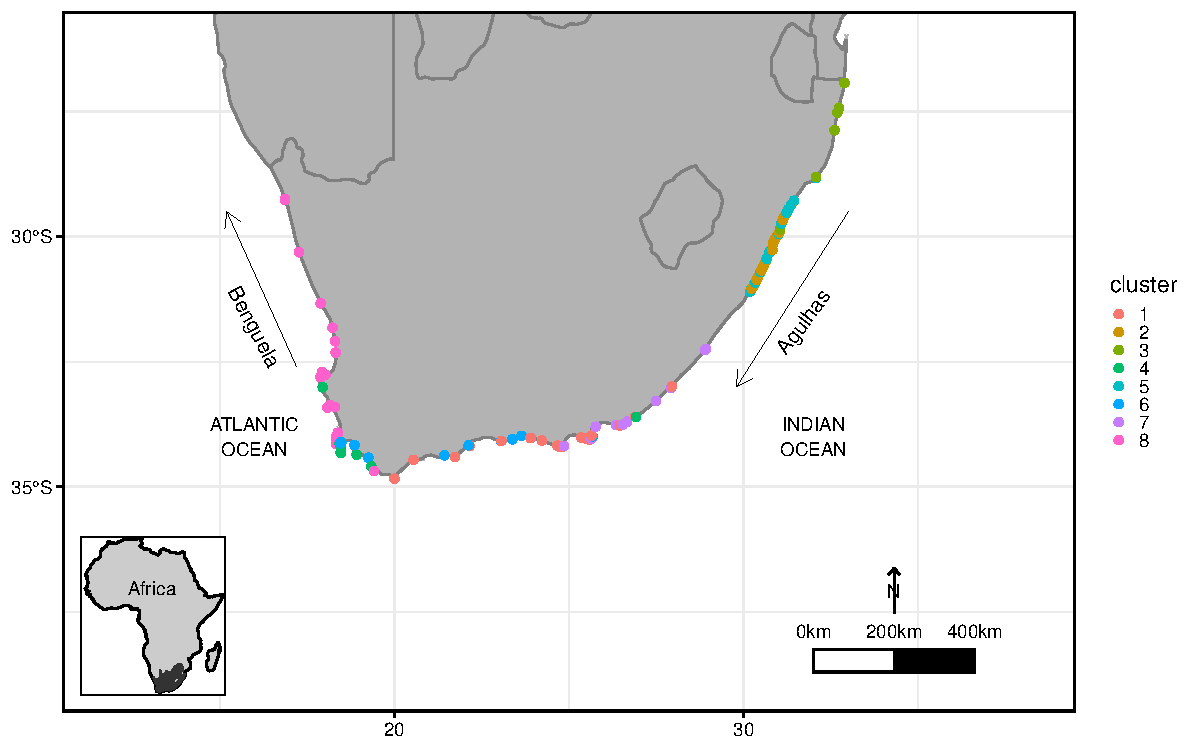
\includegraphics{../figures/map_fixed.pdf}
\caption{A map of the study area representing the 129 sites where
\emph{in situ} coastal seawater temperature was collected. These sites
were grouped based on similar mean, minimum and maximum temperatures and
as such each groups represents a unique colour variation.}
\end{figure}

Once sites were grouped together, the next step was to reduce the number
of sites down to a manageable but still representative sub-sample of the
whole. This was done for two reasons. The first was to allow for the
comparisons to be more readily interpretable by humans. Secondly it was
to allow for equal amount of sampling per coast. The east coast has
previously been more heavily sampled than the rest and such an imbalance
should be addressed. The criteria considered for the sub-samples
included selecting the longest time series within the region and
including data from as many different organizations as possible. This
process yielded three sites for each of the clusters along the South
African coastline (Figure 2). The statistical characteristics of the
temperature were used to guide analysis of the time series to produce an
accurate assessment of temperature variation between sites that were
grouped together.

\begin{figure}
\centering
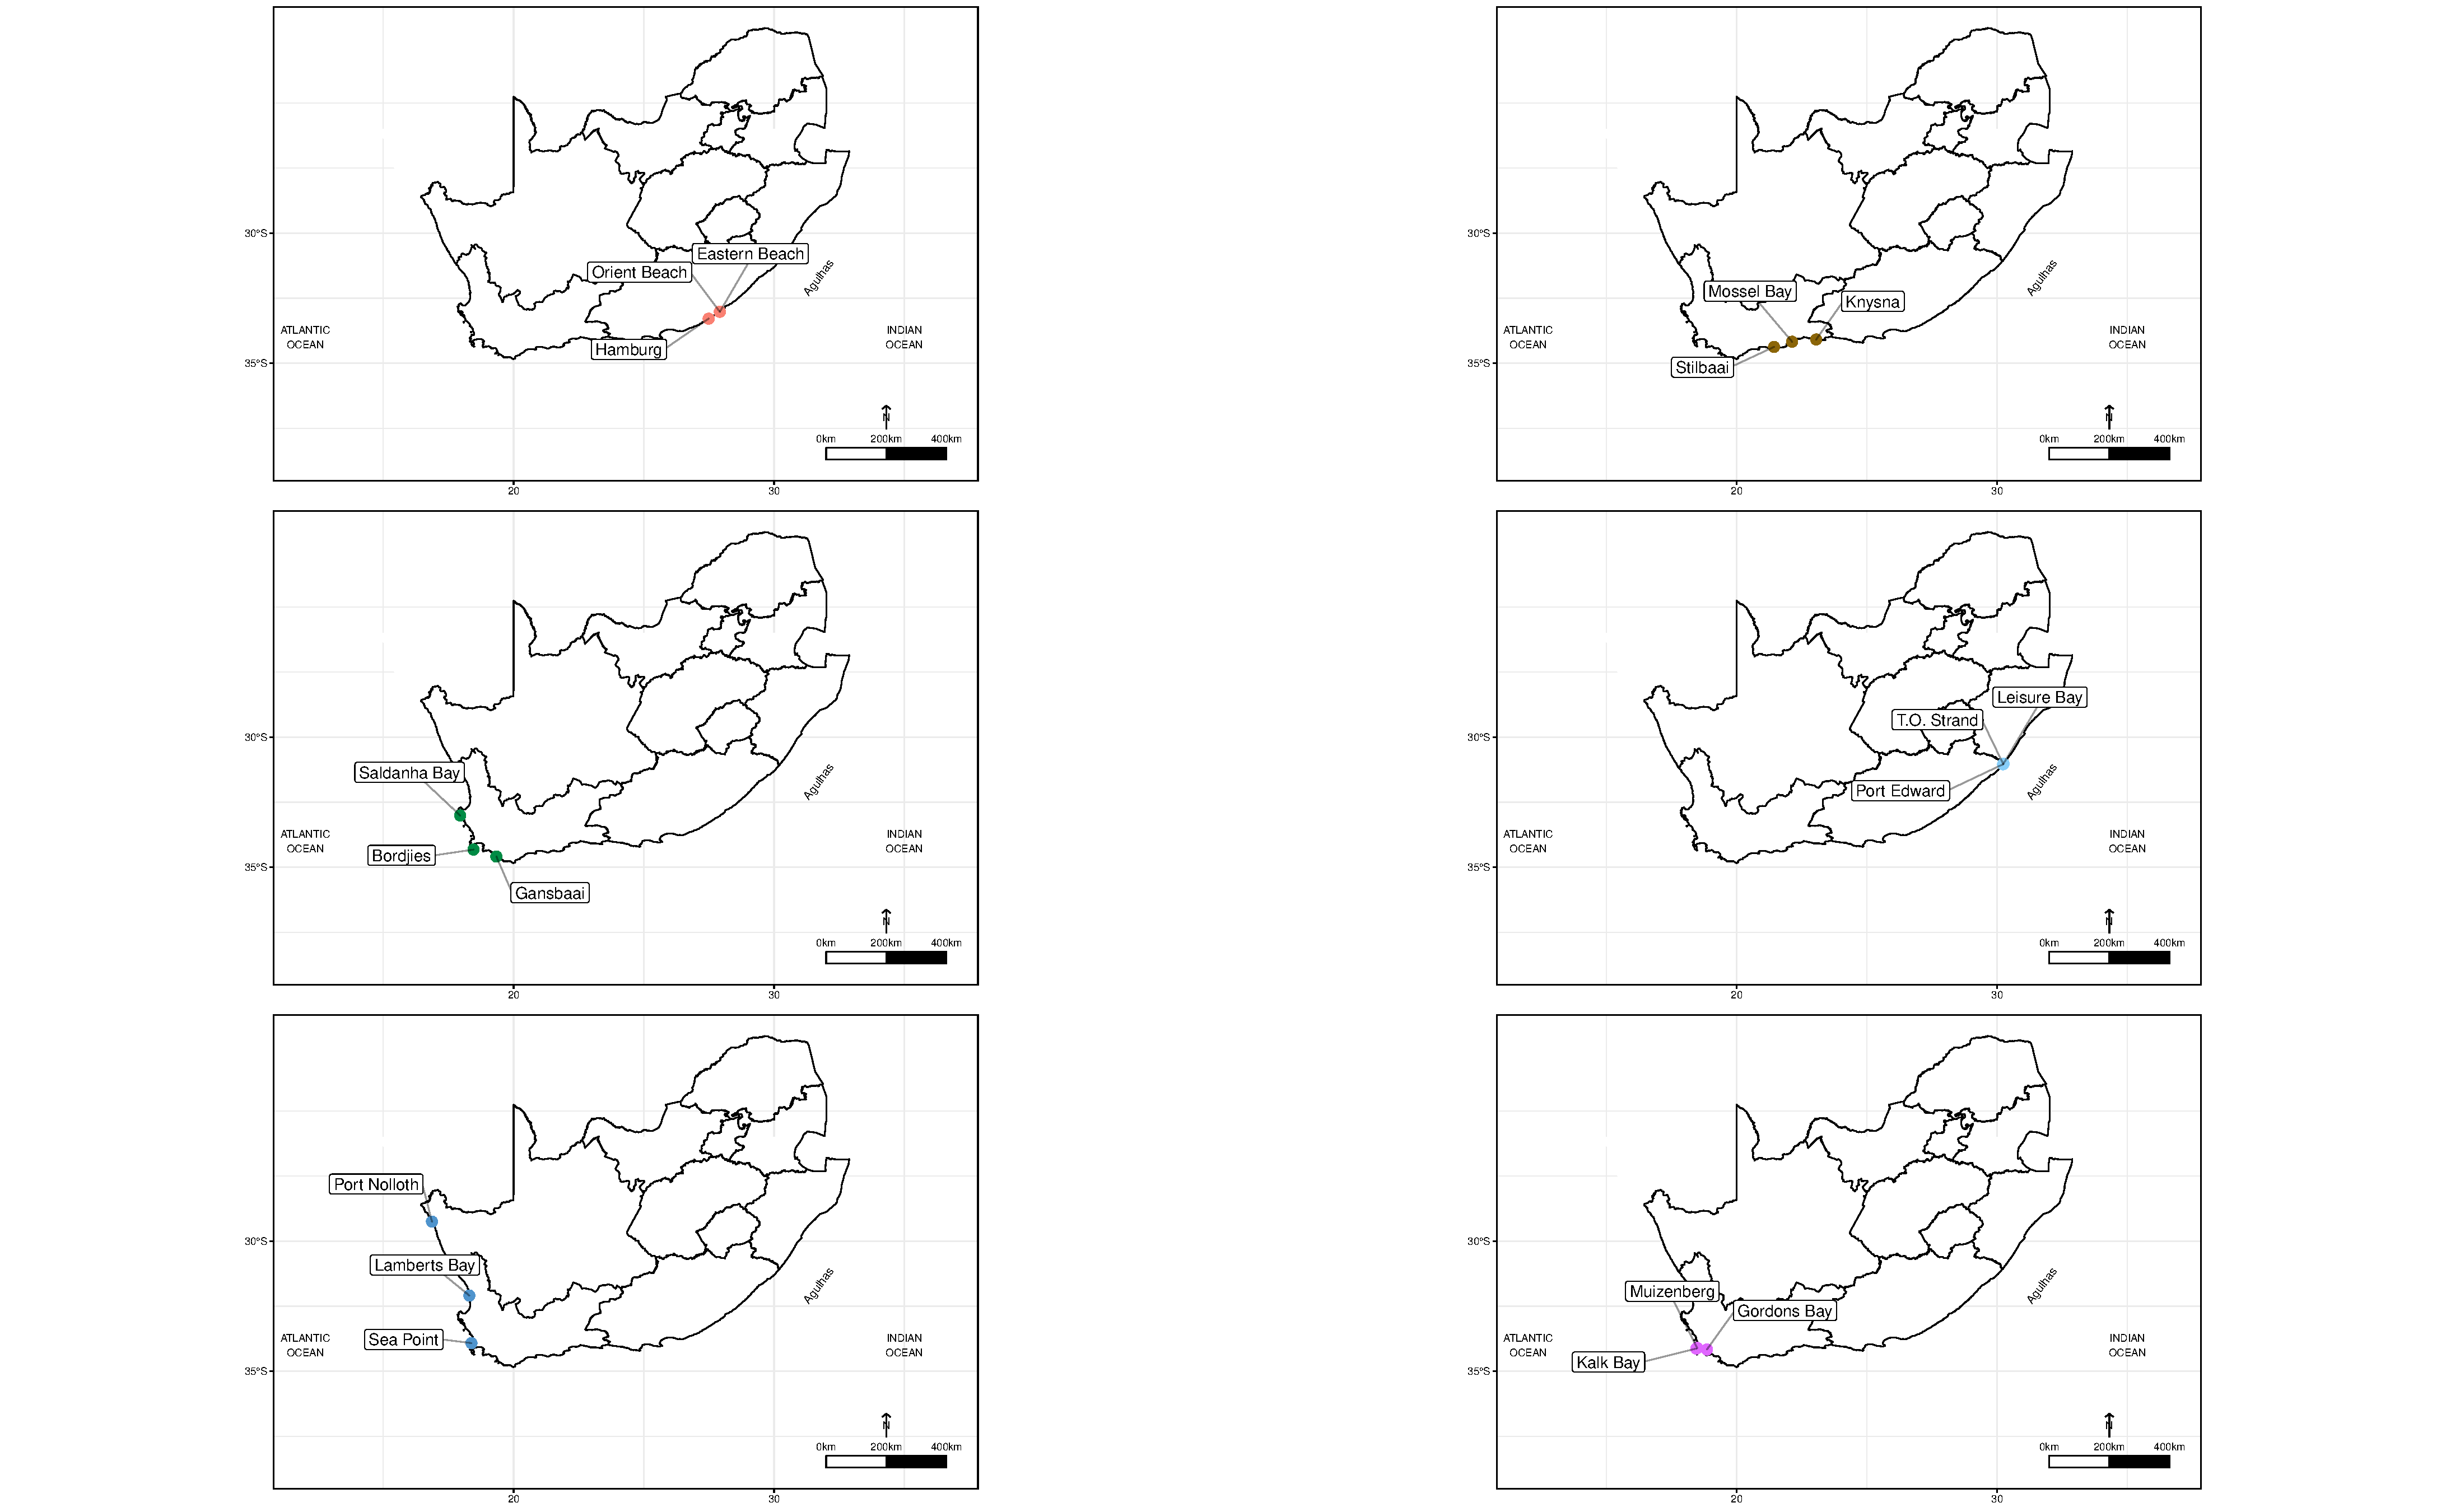
\includegraphics{../figures/final_combined_plot.pdf}
\caption{A map representing the three sites chosen within each of the
six cluster along the South African coastline.}
\end{figure}

With three sites per cluster, the haversine formula was used to
calculate the geodesic distance between points specified by radians.
Using this formula, the distances (km) between each of the sites along
the coastline were determined. Thereafter, sites within the same cluster
were matched based on the date that temperature was collected. This
allowed for a comparison to test whether or not temperature variation
exists between sites within the same cluster. Once the sites were
matched, the means and standard deviations of temperatures between sites
and clusters were determined. This highlighted the temperature variation
between matched sites and allowed for seasonal comparisons within the
same cluster.

Once the temperature variation between sites were carefully analysed,
the seawater temperature data along with the wave and wind data were
compared. The data were collected at depths of 7 m or 15 m respectively.
Since the wave and wind data were collected at three hour resolutions,
they were converted into daily data points in order to compare it with
the temperature data. The `circular' function in R software was then
used to create circular objects around the wave data in order to
calculate the daily wave and wind parameters.

With temperature and wave values now corresponding to their respective
sites, depths and dates, the hypothesis regarding whether or not a
relationship existed between wind/wave action and temperature was
tested. To do this, linear models for each site was produced, reflecting
temperature and wave variations at each depth. Linear models typically
produce coefficients of determination R2 as an output. The `purrr'
function within the `tidyverse' R package was used to simultaneously
compare temperature and wave data across sites and depths. Hereafter,
wind and wave rose diagrams were constructed to determine the most
predominant direction for a particular site. This was done to ascertain
what the potential relationship between wind/waves and temperature was
at each site during only the prevailing wind/wave directions.

\subsection{Satellite data analysis}\label{satellite-data-analysis}

Sea surface temperature measurements used in this study were obtained
from four different sources: MUR, CMC, K10 and AVHRR. A time series of
SST was determined by creating a bounding box which represented the
region of extent at the latitudes (39.5° S, 25.5°), and the longitudes
(10.5° E, 39.5° E). The size of the pixel search area was set to a 5 km
resolution from each of the stations. The satellite datasets and the
corresponding SACTN \emph{in situ} collected dataset were matched based
on the coordinates and the date at which temperature was collected. Some
sites however, shared the same satellite data due to their close
proximities. Once the satellite data corresponded to the \emph{in situ}
collected data, linear models for each site were produced, reflecting
temperature and wave variations at each depth. Linear models typically
produce coefficients of determination (R2 values) as an output, which is
the statistic showing how much of the variance in a dependent variable
is explained by the independent variable. This allows for us to test
whether or not wave and wind direction may influence temperature at the
various sites.

\subsection{Results}\label{results}

\subsection{Statistical analyses}\label{statistical-analyses}

A series of ANOVA tests were used to compare the main effects of the
chosen variables on a continuous variable. In this analysis the
relationship between matched sites based on the mean temperature as a
function of year and season were analysed, these analyses were used to
test if significant differences occured between each pair of sites
within each of the clusters. To determine the strength of correlation of
temperature between sites found within the same clusters along the
coast, boxplots were constructed. These plots enabled the visual
identification of variations in temperature by summarising the
descriptice statistics. To furthur analyse the temperature variation
between sites line graphs were constucted. This plot allowed for visual
identification of the variation in average temperature for each of the
month and year for paired sites.

\subsubsection{Temperature variation}\label{temperature-variation}

Temperatures were not uniformly distributed across the six clusters
produced (Figure 3), with each set of sites having unique patterns of
temperature variation. Cluster 1, along the south and east coast,
comprising of Hamburg, Eastern Beach and Orient Beach, it was found that
temperature varied from approximately 13 ºC to 22 ºC. Within this
cluster of sites, Hamburg had the highest maximum temperatures and the
lowest minimum temperatures of the three sites. Conversely, Orient Beach
had the lowest range of temperature variability, producing a
comparatively short box plot. Orient Beach and Eastern Beach had
relatively similar ranges and distributions of temperatures, as evident
by their box plots nearly overlapping completely.

Along the south coast, within the cluster comprised of Mossel Bay,
Stilbaai and Knysna, temperatures ranged from approximately 12 ºC to 27
ºC, with most box plots being relatively long indicating a large amount
of variation. Stilbaai had the widest range of temperature variation
among the three sites but despite the apparent differences in
temperature ranges between these sites, the average temperatures were
relatively similar. Average temperatures were nearly identical within
this cluster, with very few outliers present within the temperatures
ranges of these sites.

Sites located within the third cluster had slightly lower temperatures
than the previous two clusters. This cluster comprised of Bordjies,
Saldanha, and Gansbaai and temperatures within here ranged from
approximately 11 ºC to 21 ºC, with an average median temperature being
close to 15 ºC across all three sites. Gansbaai had relatively low
variation in temperature as it had a comparatively short box plot.
Conversely, Saldanha had a long box plot representing high variation and
relatively evenly distributed temperatures by showing little skewness.
These sites were similar in terms of their temperature, as their box
plots were largely overlapping with few differences between them. There
were however, several outliers present within the temperatures of these
sites.

The fourth cluster which was located along the east coast, comprised of
Port Edward, Leisure Bay, and T.O. Strand. Overall, the temperatures of
these sites were higher than those of the sites within the other
clusters, with a range of 15 ºC to 25 ºC. The box plots for these sites
were all decidedly long, representing a low variation of temperature
with little skewness across sites. Temperatures are they identical
between these three sites with each box plot overlapping very well . The
median temperature for each of the sites within this cluster is 20.5 ºC.

Sites within the fifth cluster had overall lower temperatures than those
within the remaining clusters. This cluster comprised of Port Nolloth,
Lamberts Bay, and Sea Point, here sharp declines in average temperatures
were observed throughout. Temperatures within this cluster ranges
between 8 ºC and 18 ºC, with an average temperature being close to 13
ºC. Port Nolloth had low variation in temperature as it had a
comparatively short box plot with relatively evenly distributed
temperatures. Lamberts Bay and Sea Point were similar in terms of
temperature variances, as their box plots were largely overlapping with
little differences between them. Several outliers were present within
the temperatures of these sites.

In the cluster comprising of Kalk Bay, Muizenberg, and Gordons Bay the
temperatures of these sites ranged from 8 ºC to 24 ºC, with most box
plots being short. Muizenberg had the widest range of temperature
variation of the three sites. Gordons Bay and Kalk Bay had identical
temperature ranges. Similarly to the second cluster, despite the
apparent differences in temperature ranges between these sites, the
average temperatures across them were relatively similar and nearly
identical.

\begin{figure}
\centering
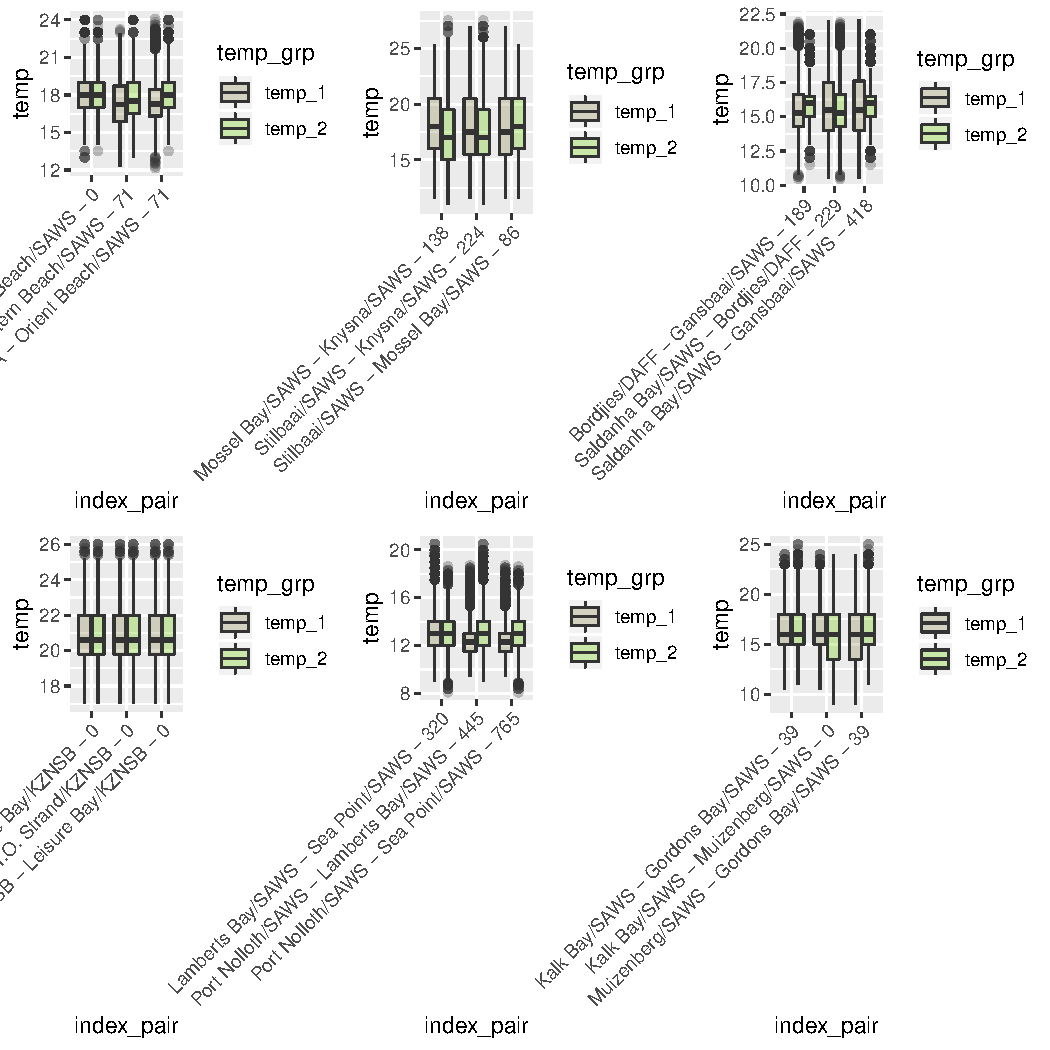
\includegraphics{../figures/combined_plot.pdf}
\caption{Boxplots representing the seawater temperature of paired sites
within each cluster along the South African coast with the values
representing the distance (km) between paired sites.}
\end{figure}

On a monthly basis, large differences of average temperatures was seen
between sites within cluster 1, comprising of Eastern Beach, Orient
Beach and Hamburg. These differences largely occured during the summer
and spring months of 1995 to 1997 (Figure 4). For the remaining sites
however, differences in average temperatures were lower during autumn.
It was also evident that the average temperature between Hamburg and
Orient Beach varied largely on an apparent seasonal basis. Small monthly
average temperature differences existed between Eastern Beach and Orient
Beach throughout the different seasons.

Converse to the first cluster, the cluster containing Mossel Bay, Knysna
and Stilbaai, the largest differences in average temperatures were
observed during spring. In this cluster large differences in average
temperatures were present between Mossel Bay and Knysna, with the
differences increasing annually from 1985 to 2017. Similarly,
differences in average temperature also increased slightly between
Stilbaai and Knysna during winter and spring. During summer months
little differences in average temperature were seen between all three
sites within this cluster.

Differences of average temperatures between sites within cluster 3
(Bordjies, Gansbaai and Saldahna Bay) varied on a seasonal basis. During
the summer months, large differences in average temperatures exist
between Bordjies and the remaining twonsites, with an increase in
differences of average temperature between Saldanha Bay and Gansbaai
throughout autumn, winter and spring.

In the fourth cluster, which comprised of Port Edward, Leisure Bay and
T.O. Strand, small changes in the differences of monthly average
temperatures were noticed between sites between 1980 to 2017. Here, the
large differences in temperatures were observed towards the end of
spring and during summer months. Temperatures were relatively stable
throughout winter and the beginning of spring across all three sites
found within this cluster.

In the cluster comprising of Lamberts Bay, Port Nolloth and Sea Point,
large differences in average temperatures existed between sites at
selected months between 1972 and 2017. During summer and autumn months,
differences in average temperature were observed between Lamberts Bay
and the remaining sites increased. During the months of autumn Lamberts
Bay and Sea Point showed large differences in average temperature
variation. For the remaining sites, differences in average temperatures
were relatively low throughout each month for the same time period.

In the cluster comprising of Kalk Bay, Gordons Bay and Muizenberg, the
largest differences in average temperatures were observed during mid
autumn and winter months. In this cluster large differences in average
temperatures were seen between Muizenberg and the remaining sites, with
the differences increasing annually throughout 1972 and 2016 during
winter. Similarly, differences of average temperatures also increased
between Kalk Bay and Muizenberg during these same months. In the summer
and spring months little differences in average temperatures between
sites, with minimal differences in the rates of these changes. These
rates increased during spring.

\begin{figure}
\centering
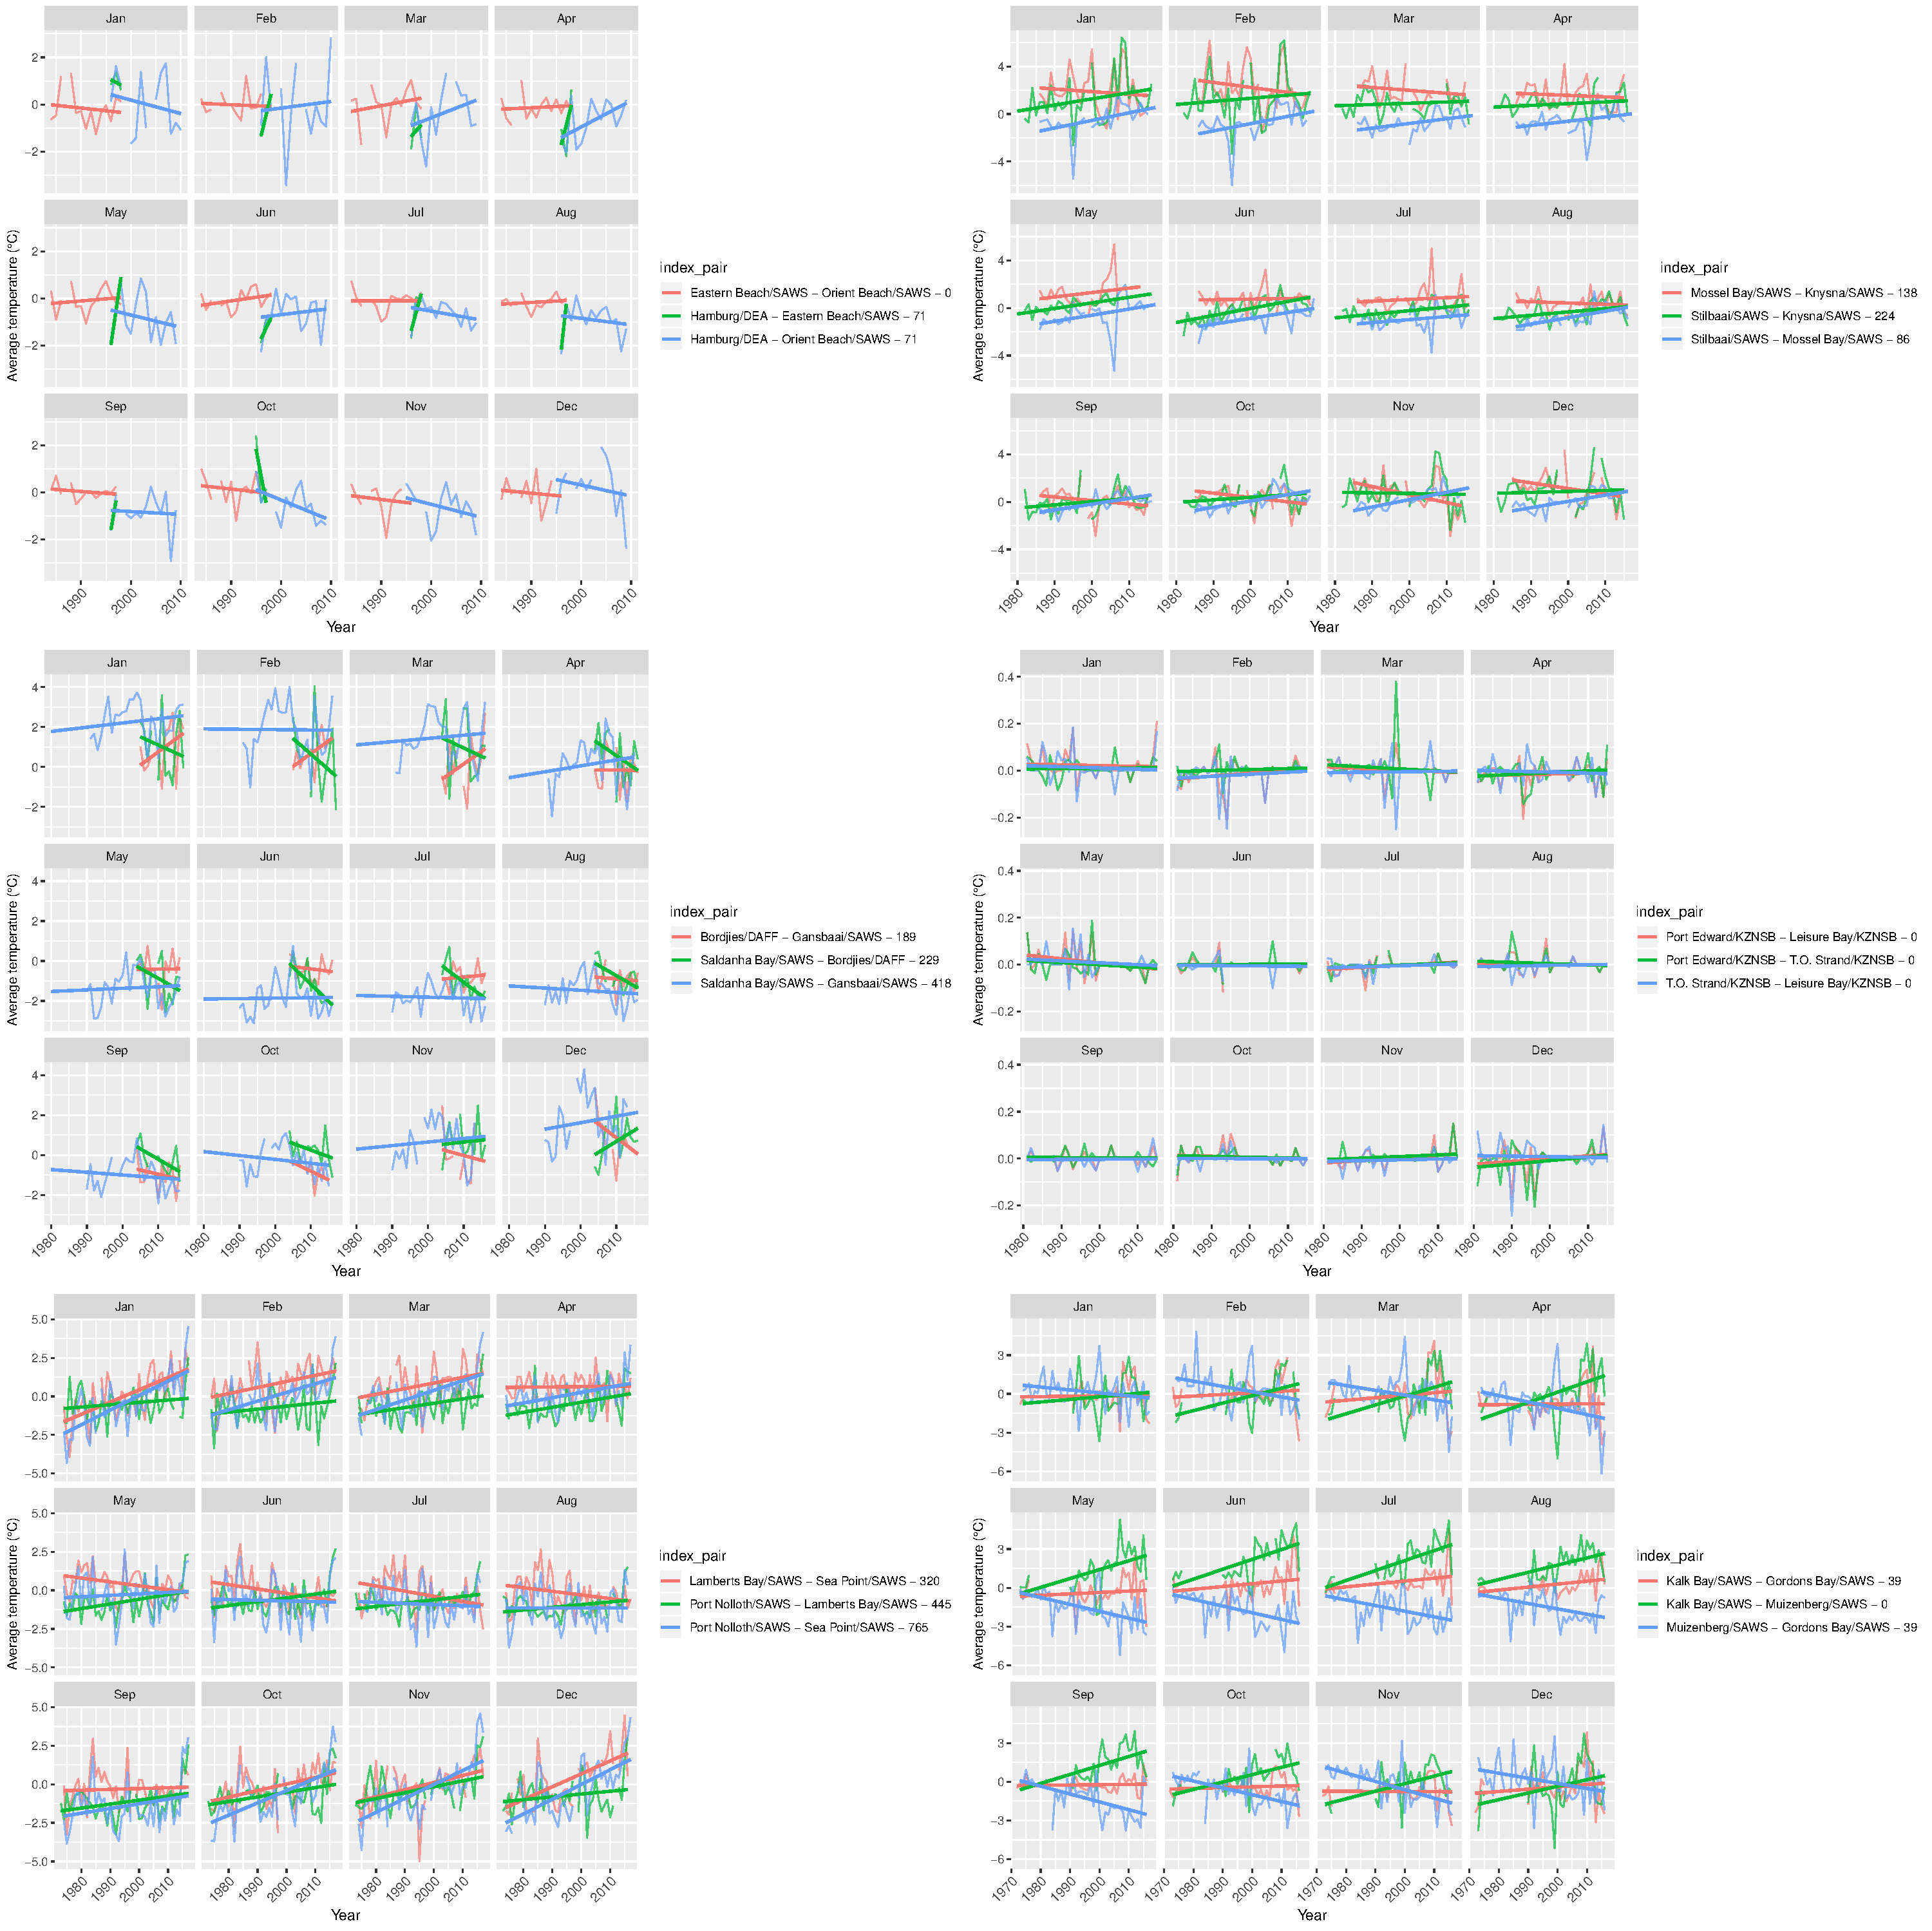
\includegraphics{../figures/figures/combined2_plot.pdf}
\caption{Line graph representing the variation in average seawater
temperature for each of the month and year for paired sites along the
South African coastline with the values representing the distance (km)
between paired sites.}
\end{figure}

\subsubsection{Average temperature of clustered
sites}\label{average-temperature-of-clustered-sites}

In the first cluster of sites, the results of a one way ANOVA tests it
was found that there was a significant (p \textless{} 0.05) differences
in average temperatures between paired sites (F = 12.07, SS = 15.28, p
\textless{} 0.001). These differences were present across season (F =
3.44, SS = 13.07, p \textless{} 0.002) but were not present yearly
between individual sites and paired sites (F = 1.38, SS = 1.75, p =
0.25). Similarly, paired sites within the second cluster also a
significantly differed in average temperature (F = 166.84, SS = 418.6, p
\textless{} 0.001). Conversely to first cluster however these
differences were present yearly (F = 33.21, SS = 41.7, p \textless{}
0.001) and seasonally (F = 16.72, SS = 125.9, p \textless{} 0.02,)
between individual and paired sites. In the third cluster of sites,
ANOVA tests revealed that there were no significant differences in
average temperatures between paired sites (F = 1.17, SS = 2.9, p =
0.31), but temperatures varied seasonally and yearly between individual
sites. In the fourth cluster there were again no significant difference
of average temperatures between paired sites (F = 0.73, SS = 2.9, p =
0.48). Significant differences were also absent across seasons (F =
0.75, SS = 0.0042, p = 0.52) and years (F = 0.495, SS = 0.0009, p =
0.48) between both individual and paired sites. Sites within the fifth
cluster were significantly different in average temperatures between
paired sites (F = 77.10, SS = 196.7, p \textless{} 0.002), with these
differences being present yearly (F= 172.80, SS = 220.4, p \textless{}
0.001) and seasonally (F = 77.10, SS = 29.92, p \textless{} 0.002) for
both paired and individual sites. Finally, sites within the sixth
cluster also significantly difference in average temperatures between
paired sites, yearly and seasonally (F = 132.044, SS = 419.7, p
\textless{}0.01).

\subsection{The impact of wind and wave action on
temperature}\label{the-impact-of-wind-and-wave-action-on-temperature}

\subsection{SACTN dataset:}\label{sactn-dataset}

The coeffcient of determination was calculated to analyse how
differences in one variable can be explained by a difference in the
second variable. Here, the relationship between temperature and several
variables including wind direction and speed as well as wave height,
period, direction and speed was determined for all 18 sites. The results
showed little variation in environmental factors and temperature for
each of the sites. Wind and wave direction influenced temperature at 0
-- 3\%. The most significant relationships were found in Muizenberg,
Kalk Bay and Mossel Bay where the R\^{}2 values indicated that wave
period had a 6-7\% influence on temperature. Overall wind and wave
action had no significant impact on temperature differences along the
coast.

\subsection{Satellite dataset}\label{satellite-dataset}

Upon examining the impact of wind and wave action on seawater
temperature of the AVHRR temperature dataset, it was seen that wave and
wind direction had a minimal effect on temperature variation with its
R\^{}2 values ranging between 0-3\%. The results also indicated that
wave height influenced temperature at some of the sites. This was
evident in Gaansbaai and Lamberts Bay where wave height had a 9\% impact
on temperature variation. The results obtained from the MUR dataset
continued to show little variation in regards to the influence of wind
and wave action on temperature. At many of the sites, both wind and wave
direction had a 0\% impact on the temperature, however, it was seen that
wave height and wave period had the greatest impact on temperature at
some of the sites, with Gordons Bay and Gaansbaai indicating an 8\% and
10\% impact of wave height on temperature variation respectively. The
results obtained from the CMC temperature dataset indicated that wave
and wind direction as well as wind speed showed the least significant
impact on temperature variation with r\^{}2 values ranging between
0-3\%. Wave height continued to show the largest impact on temperature
variation at some of the sites. Gaansbaai and Gordons Bay indicated the
highest R\^{}2 values of 12\% and 9\% respectively. Upon comparing the
impact of various environmental factors on temperature variation for the
K10 data, the results indicated that the each of the above-mentioned
variables had no impact on the temperature variation at Hamburg. The
impact of wind direction on temperature is highest at Gansbaai,
representing an R\^{}2 value of 4\% while wave height still repersented
the greatest influence on temperature occurring at these sites.

\subsection{Wind rose diagram}\label{wind-rose-diagram}

Wind and wave diagrams help visualise the patterns present at a
particular site. As you move outward on the radial scale, the frequency
associated with wind and waves coming from a partiular direction
increases. The predominant wind direction along the south coast
105degrees. The predominant wind direction of sites located along the
east coast such as T.O. Strand and Orient Beach occured at 45 degrees.
Leisure Bay, also located along the east coast however indicates a
predominant wind direction of 15degrees. Port Nolloth, located along the
west coast, indicates a predominant wind direction at both 135 degrees
and 165 degrees.

\begin{figure}
\centering
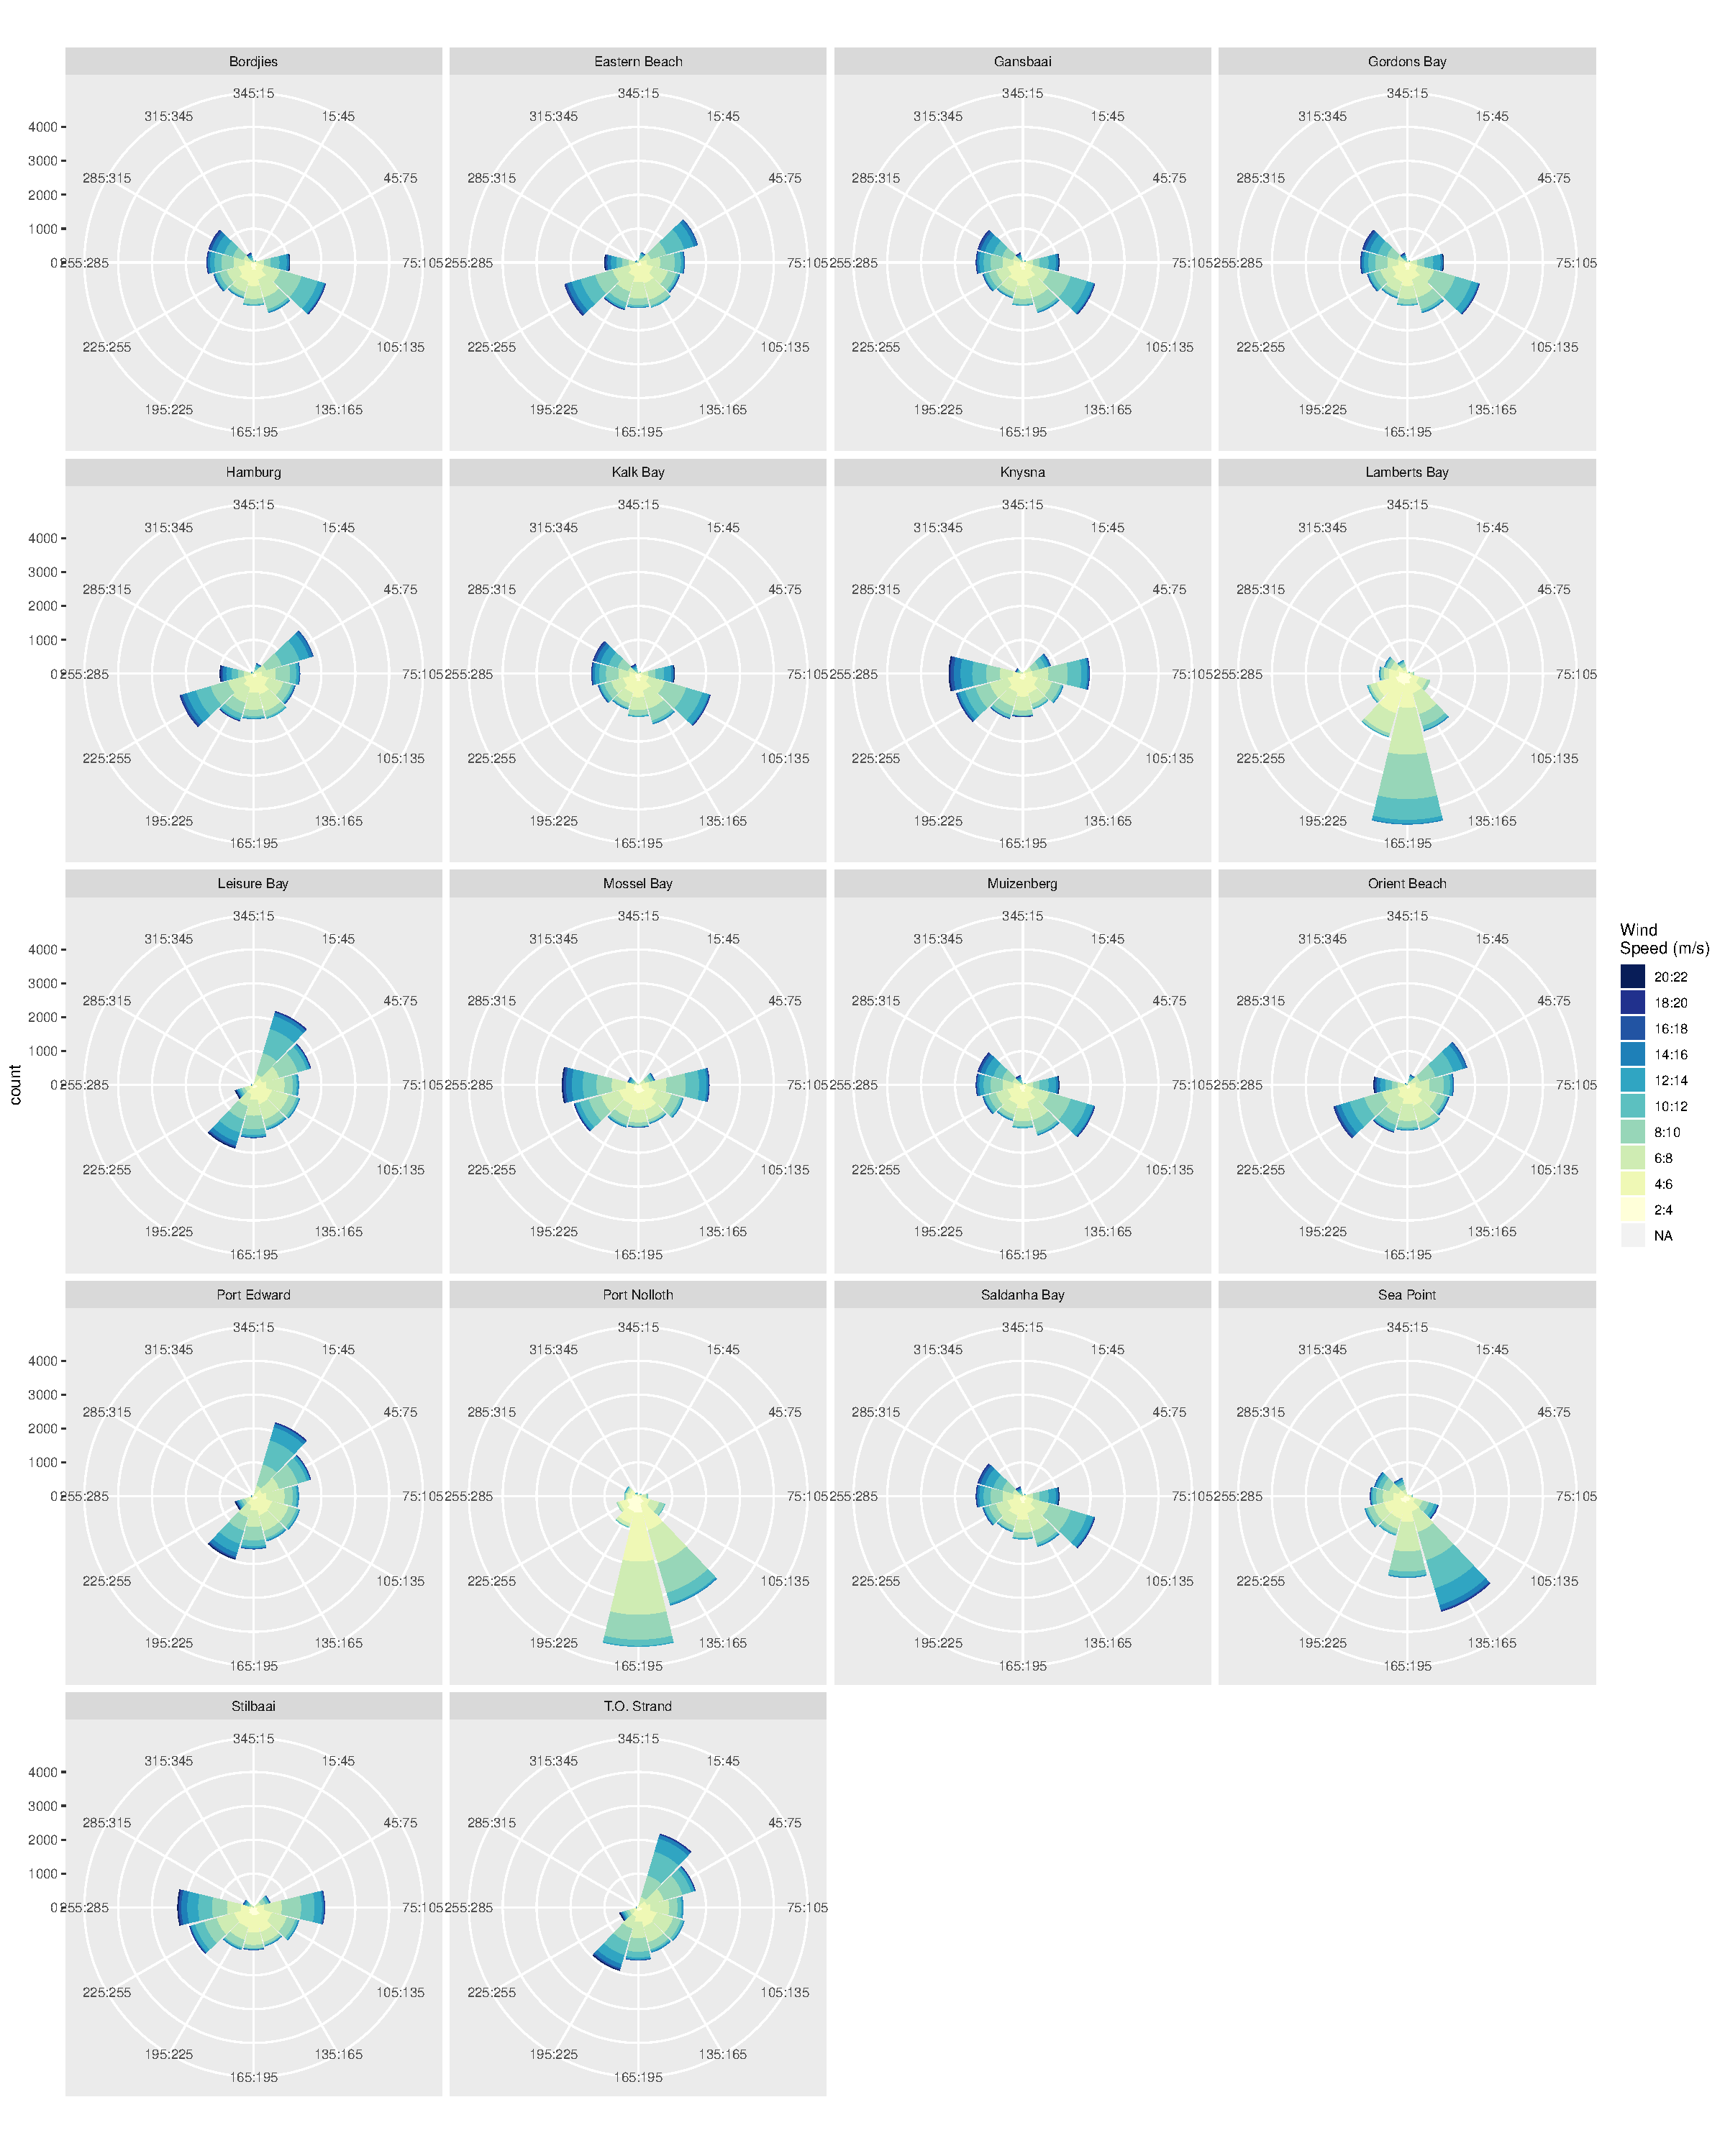
\includegraphics{../figures/p.wr3.pdf}
\caption{Wind rose diagrams representing the the most predominant wind
direction for each of the sites. Each spoke is divided by color into
wind speed ranges. The radial length of each spoke around the circle is
the time that the wind and waves comes from that direction}
\end{figure}

\subsection{The impact of predominant wind and wave action on seawater
temperature}\label{the-impact-of-predominant-wind-and-wave-action-on-seawater-temperature}

The results indicated that wind speed, wind height, wind and wave
direction as well as wave period had no significant impact on \emph{in
situ} temperature variation at the various sites along the coastline
(Figure 6). Eastern Beach however, showed that wave period and wave
height appear to have the largest effect on temperature variation, this
however varied between sites. Hamburg and Gordons Bay show that wave
direction explained 4\% of the temperature variation. Muizenberg,
representing the largest value of 5\% influence of wave height on
temperature variation. Cluster two comprising of Stilbaai, Mossel Bay
and Knysna, wind and wave action had very little impact on temperature
variation, with all three graphs representing similar results. In the
cluster comprising of Port Edward, Leisure Bay and T.O Strand, wave
height is seen to have a minor impact on temperature variation with an
r-squared value variating between 1-5\%. Overall it is seen that
predominant wind and wave direction have no significant impact on the
seawater temperature variation along the coast.

\begin{figure}
\centering
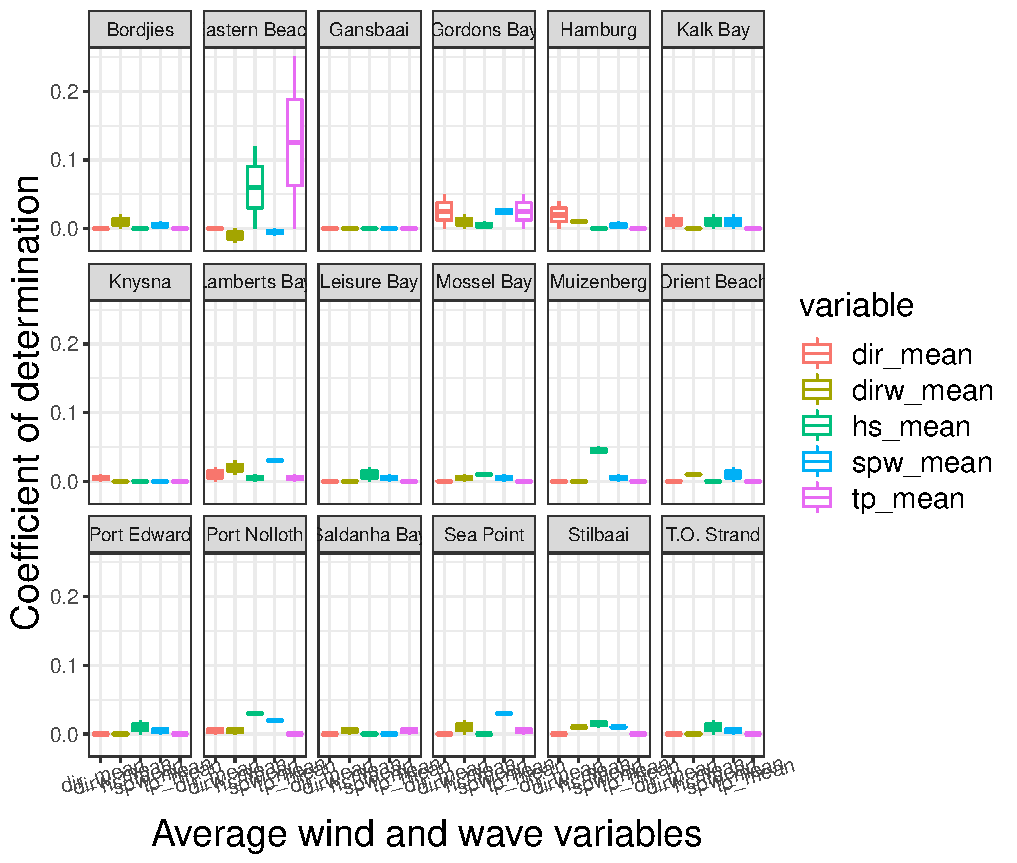
\includegraphics{../figures/predominant_ww.pdf}
\caption{Boxplot representing the adjusted r\^{}2 value each of the
environmental variables at the most predominant wave and wind direction
for each of the sites.}
\end{figure}

\subsection{Discussion}\label{discussion}

\textcolor{red}{why was it expected that wind and wave may influece tempeature}

This study aimed to investigate how wind and wave action influenced
variation in coastal seawater temperature along the South African
coastline. As seawater temperature is known to have large influences on
species distributions (Bolton 2010; Smit et al. 2013), it is important
to understand not only how temperatures vary along the coastline, but
the factors driving these variations as well. Sinnett and Feddesen
(2014) proved that various environmental factors such as solar
radiation, air temperature, humidity and wave energy is responsible for
temperature variation within the coastal region. Here, It was confirmed
that there were statistically significant differences in the \emph{in
situ} seawater temperature between 18 sites along the coastline of South
Africa, with temperatures contrasting between coasts, and among sites
along the same coasts. Overall, sites located along the west coast had
lower temperatures than those along the south and east coasts. It was
discovered that the east coast had overall, little variation in
temperatures between sites, whereas the south coast varied more
frequently (Schlegel and Smit 2016).

The results in this study confirmed that there were significant
differences in temperatures between sites along the coastline, annually
and seasonally, but did not provide evidence of which factors were
driving these. Across each of the 18 sites that were assessed, it was
found that wind and wave action did not significantly influence both
satellite and \emph{in situ} SSTs. Differences in temperature between
sites at different locations along the coastline were therefore not
caused by variations in wind or wave action, suggesting that other
factors were responsible for the observed patterns of temperature
variation. These findings were consistent across six different datasets
from various sources, with each of these providing minimal evidence of a
relationship between wind or wave action and the SST of a site. It must
be noted however, these analyses consisted of a combination of satellite
and thermometer data, which varied in their measurements and time
series.

Theron et al. (2014) discusses how the wave data set, from which the
current study data was extracted from, was created and validated.
However, despite the validation, discrepaancies may arise as a result of
the assumptions made in the assumptions of the SWAN model.
Quasi-stationary SWAN computation were performed under the assumption
that the boundary conditions were fluctuating at a much slower tempo
compare to the time it took for those conditions to propagate towards
the coastline. This may ultimately result in the wind driven wave
components to be overestimated as the duration limited effect of the
wind was thus neglected and computed towards a converging wave condition
during each quasi-stationary time step.

The SWAN model usually overestimates the energy of developing waves with
low frequencies (long periods) for very short distances from the shore.
This is because wave conditions are simplified by using an a priori wave
spectrum (Booij, Ris, and Holthuijsen 1999; Thomas and Dwarakish 2015).
For most modelled areas, these assumptions are reasonable to make
because most of the South African coastline is exposed and agree to the
requirements of these assumptions (Joubert et al. 2013).

Previous studies suggest that a longer time series containing more data
would have greater accuracy in detecting subtle changes in temperature
differences obtained from variable coastal regions such as the South
African coastline. Schlegel and Smit (2016) suggested that having a time
series of greater than 30 years for sites with a low variance results in
increased ability to detect changes. They showed that high quality time
series datasets have frequent measurements with minimal missing (NA)
values present. Furthermore, low quality datasets (i.e.~those with more
than 5\% of NA values) have a higher chance of detecting variation where
none exists.

The SACTN dataset containing temperature information are inconsistent.
Temperature collection along the South African coastline started in the
1970s, and has been inconsistent in terms of instruments used,
modifications to styles and methods, calibration, and site locations
(Smit et al. 2013; Schlegel and Smit 2016). Additionally, older records
within some datasets, such as the SACTN dataset, may have been lost or
are unreliable since the metadata for these are unavailable. These
metadata are essential as their absence prevents the understanding of
the influence that the instruments had on temperature recordings. Some
measurements may therefore not represent accurate temperatures due to
the instrumentation used however, have an accurate indication of which
recordings were measured with thermometers and which were with UTRs is
available.

The UTRs used to collect data in the SACTN dataset appeared to express a
lower number of NA values compared to the data collected with hand
thermometers. As such, this may have influenced the overall time series
dataset (Schlegel and Smit 2016). The level of precision at which data
was collected also influenced the length of the time series needed. Time
series in which temperature were collected at a precision of 0.5 ºC may
require another 24 months of recordings to precisely detect long term
variation (Schlegel and Smit 2016). The average length of the
thermometer time series component of the SACTN dataset was 346 months
whereas the average length of UTR time series was less than half of
that. With the extent of these differences in length being so severe,
even once correcting for potential negative effects on the measurement
precision of the thermometer collected time series, it was clear that
thermometer data were more useful than that of UTRS.

Satellite acquired SST records are useful to modern marine scientists.
These data are often used to model and predict a wide range of oceanic
and biological processes in the open ocean but have only recently been
used to study temperature variations influencing benthic organisms
(Pearce, Faskel, and Hyndes 2006). Here, both satellite SST data, and in
situ thermometer data were correlated with wind and wave data along the
coastal environment at a depth of 7 and 15 meters respectively. SST data
acquired by satellites are obtained from a thin boundary layer at the
air-sea interface ({\textbf{???}}) and at different locations and thus
deviated from coastal in situ collected seawater temperatures. These
deviations may have affected the outcomes of the analyses thereby
inhibiting the findings. Upon assessing the impacts of wind and wave
action on satellite and in situ collected seawater temperature data it
was found that wind and wave action had insignificant impacts on the
temperature variation along the South African coastline.

My findings were surprising but not unexpected. Along the coastline of
South Africa, there is a known east-west thermal temperature gradient
that may have caused some interesting results (Smit et al. 2013). This
is caused by major oceanic processes such as coastal upwelling,
thermohaline circulation, solar radiation, atmospheric temperature
({\textbf{???}}) and the presence of major ocean currents, which
cumulatively influences the temperatures along this coastline
({\textbf{???}}; Schlegel and Smit 2016). While it was reasonable to
assume that surface level environmental factors like wind and wave
action would affect sea surface temperatures, it is not completely
unexpected that they would have little effect given the prevalence of
the major processes mentioned above. However, this is unlikely as the
`West Coast' system is considered wind driven and there are multiple
wind driven upwelling cells along the south coast. Those processes are
of the largest drivers behind coastal temperature variation and may
simply be overpowering the effects of other environmental factors. Other
factors such as latent heat flux and wave energy flux were also proven
to heat and cool coastal seawater temperatures ({\textbf{???}}).

Alternatively, it is possible that factors other than wind and wave
action are influencing temperatures across the South African coastline.
For example, whilst rainfall can have large influences on coastal SST
(Reason and Mulenga 1999) other, non-climatic, factors could be playing
a greater role. Coastal regions are highly impacted by human mediated
pressures (A Mead et al. 2013). These pressures are predicted to drive
change over a spatial and temporal scale and is often a cause of
temperature variation (Griffiths, Mead, and Zietsman 2011).
Additionally, evidence indicates that human driven climate change on
both a local and global scale largely influence seawater temperatures,
wind regimes, and wave action ({\textbf{???}}; M. J. Rouault et al.
2010; A Mead et al. 2013). These pressures are present along the South
African coastline in the form of pollution, coastal runoff, invasive
species, resource exploitation, and coastal mining, which directly and
indirectly influences air temperature, wind, seawater temperature, and
rainfall ({\textbf{???}}; James and Hermes 2011; A Mead et al. 2013).
These anthropogenic factors may be cumulatively playing an important
role in affecting SST along the coastline, but the full extent of these
factors are unknown.

Within marine environments, coastal temperature variation allows for a
variation in the spatial arrangements of marine biodiversity. Whilst
wind and wave action may not be directly affecting ocean temperatures,
Blamey and Branch (2008) have found that wave action has a profound
influence on species distributions along the coastline. The presence or
absence of marine species are determined by a variety of factors and
whilst those factors may not be influencing each other as was the case
here, they collectively play important roles in affecting the marine
life of the South African coastline and identifying those roles can aid
in improving our understanding of nearshore dynamics, thereby providing
greater knowledge to be used for conservation.

This study has shown that wind and wave action are not directly
affecting seawater temperature variation along the South African
coastline, However, other factors may be. Future research could aim to
examine the effects of air temperature and rainfall on the coastal
seawater temperature for the 18 sites being assessed. Additionally,
other factors such as the amount of sunlight penetrating the ocean or
site exposure could also be tested, as well as assessing the optimal
locations for data collection. Further studies should also consider
examining how chlorophyll concentrations and salinity varies with
temperature in order to assess the effects of seawater temperature on
marine plant life. Homogenous coastlines with distinct temperature
gradients such as in South Africa provide a model environment for
temperature analyses at fine-resolutions. These data could provide
critically important information that can be used to assist in
conserving marine biodiversity within these waters and should be given
greater priority within marine research in the near future.

\hypertarget{refs}{}
\hypertarget{ref-Bartsch2012}{}
Bartsch, Inka, Christian Wiencke, and Thomas Laepple. 2012. ``Global
Seaweed Biogeography Under a Changing Climate: The Prospected Effects of
Temperature.'' In \emph{Seaweed Biology}, 383--406. Springer.

\hypertarget{ref-Beal2011}{}
Beal, Lisa M, Wilhelmus PM De Ruijter, Arne Biastoch, Rainer Zahn,
Meghan Cronin, Juliet Hermes, Johann Lutjeharms, et al. 2011. ``On the
Role of the Agulhas System in Ocean Circulation and Climate.''
\emph{Nature} 472 (7344). Nature Publishing Group: 429.

\hypertarget{ref-Bolton2004}{}
Bolton, JJ, Frédérik Leliaert, Olivier De Clerck, RJ Anderson, H
Stegenga, HE Engledow, and Eric Coppejans. 2004. ``Where Is the Western
Limit of the Tropical Indian Ocean Seaweed Flora? An Analysis of
Intertidal Seaweed Biogeography on the East Coast of South Africa.''
\emph{Marine Biology} 144 (1). Springer: 51--59.

\hypertarget{ref-Bolton2010}{}
Bolton, John J. 2010. ``The Biogeography of Kelps (Laminariales,
Phaeophyceae): A Global Analysis with New Insights from Recent Advances
in Molecular Phylogenetics.'' \emph{Helgoland Marine Research} 64 (4):
263.

\hypertarget{ref-Booij1999}{}
Booij, NRRC, RC Ris, and Leo H Holthuijsen. 1999. ``A Third-Generation
Wave Model for Coastal Regions: 1. Model Description and Validation.''
\emph{Journal of Geophysical Research: Oceans} 104 (C4). Wiley Online
Library: 7649--66.

\hypertarget{ref-Breeman1988}{}
Breeman, AM. 1988. ``Relative Importance of Temperature and Other
Factors in Determining Geographic Boundaries of Seaweeds: Experimental
and Phenological Evidence.'' \emph{Helgoländer Meeresuntersuchungen} 42
(2): 199.

\hypertarget{ref-Broitman2008}{}
Broitman, BR, CA Blanchette, BA Menge, J Lubchenco, C Krenz, M Foley, PT
Raimondi, D Lohse, and SD Gaines. 2008. ``Spatial and Temporal Patterns
of Invertebrate Recruitment Along the West Coast of the United States.''
\emph{Ecological Monographs} 78 (3). Wiley Online Library: 403--21.

\hypertarget{ref-Byrne2009}{}
Byrne, Maria, Melanie Ho, Paulina Selvakumaraswamy, Hong D Nguyen, Symon
A Dworjanyn, and Andy R Davis. 2009. ``Temperature, but Not pH,
Compromises Sea Urchin Fertilization and Early Development Under
Near-Future Climate Change Scenarios.'' \emph{Proceedings of the Royal
Society of London B: Biological Sciences} 276 (1663). The Royal Society:
1883--8.

\hypertarget{ref-Davis2011}{}
Davis, KA, SJ Lentz, J Pineda, JT Farrar, VR Starczak, and JH Churchill.
2011. ``Observations of the Thermal Environment on Red Sea Platform
Reefs: A Heat Budget Analysis.'' \emph{Coral Reefs} 30 (1). Springer:
25--36.

\hypertarget{ref-Easterling2000}{}
Easterling, David R, Gerald A Meehl, Camille Parmesan, Stanley A
Changnon, Thomas R Karl, and Linda O Mearns. 2000. ``Climate Extremes:
Observations, Modeling, and Impacts.'' \emph{Science} 289 (5487).
American Association for the Advancement of Science: 2068--74.

\hypertarget{ref-Fewings2011}{}
Fewings, Melanie R, and Steven J Lentz. 2011. ``Summertime Cooling of
the Shallow Continental Shelf.'' \emph{Journal of Geophysical Research:
Oceans} 116 (C7). Wiley Online Library.

\hypertarget{ref-Griffiths2011}{}
Griffiths, CL, A Mead, and L Zietsman. 2011. ``Human Activities as
Drivers of Change on South African Rocky Shores.'' \emph{Observations on
Environmental Change in South Africa, Sun Media, Stellenbosch, South
Africa}, 242--6.

\hypertarget{ref-Hoek1982}{}
Hoek, C van den. 1982. ``The Distribution of Benthic Marine Algae in
Relation to the Temperature Regulation of Their Life Histories.''
\emph{Biological Journal of the Linnean Society} 18 (2). Wiley Online
Library: 81--144.

\hypertarget{ref-Hutchings2009}{}
Hutchings, L, CD Van der Lingen, LJ Shannon, RJM Crawford, HMS Verheye,
CH Bartholomae, AK Van der Plas, et al. 2009. ``The Benguela Current: An
Ecosystem of Four Components.'' \emph{Progress in Oceanography} 83
(1-4). Elsevier: 15--32.

\hypertarget{ref-James2011}{}
James, Nicola Caroline, and Juliet Hermes. 2011. \emph{Insights into
Impacts of Climate Change on the South African Marine and Coastal
Environment}. SAEON.

\hypertarget{ref-Joubert2013}{}
Joubert, JR, JL van Niekerk, J Reinecke, and I Meyer. 2013. ``Wave
Energy Converters (Wecs).'' \emph{Centre for Renewable and Sustainable
Energy Studies, Centre for Renewable and Sustainable Energy Studies,
Faculty of Engineering}.

\hypertarget{ref-Lee2018}{}
Lee, Kate Asha, Moninya Roughan, Hamish Malcolm, and Nicholas Otway.
2018. ``Assessing the Use of Area-and Time-Averaging Based on Known
de-Correlation Scales to Provide Satellite Derived Sea Surface
Temperatures in Coastal Areas.'' \emph{Frontiers in Marine Science} 5.
Frontiers: 261.

\hypertarget{ref-Lutjeharms1988}{}
Lutjeharms, JRE, and RC Van Ballegooyen. 1988. ``Anomalous Upstream
Retroflection in the Agulhas Current.'' \emph{Science} 240 (4860). The
American Association for the Advancement of Science: 1770.

\hypertarget{ref-Lutjeharms2000}{}
Lutjeharms, JRE, J Cooper, and M Roberts. 2000. ``Upwelling at the
Inshore Edge of the Agulhas Current.'' \emph{Continental Shelf Research}
20 (7). Elsevier: 737--61.

\hypertarget{ref-Luning1990}{}
Lüning, Klaus. 1990. \emph{Seaweeds: Their Environment, Biogeography,
and Ecophysiology}. John Wiley \& Sons.

\hypertarget{ref-Mead2013}{}
Mead, A, CL Griffiths, GM Branch, CD McQuaid, LK Blamey, JJ Bolton, RJ
Anderson, et al. 2013. ``Human-Mediated Drivers of Change---impacts on
Coastal Ecosystems and Marine Biota of South Africa.'' \emph{African
Journal of Marine Science} 35 (3). Taylor \& Francis: 403--25.

\hypertarget{ref-Mead2011}{}
Mead, Angela. 2011. ``Climate and Bioinvasives Drivers of Change on
South African Rocky Shores?'' PhD thesis, University of Cape Town.

\hypertarget{ref-Meehl2004}{}
Meehl, Gerald A, and Claudia Tebaldi. 2004. ``More Intense, More
Frequent, and Longer Lasting Heat Waves in the 21st Century.''
\emph{Science} 305 (5686). American Association for the Advancement of
Science: 994--97.

\hypertarget{ref-Muller2009}{}
Müller, Ruth, Thomas Laepple, Inka Bartsch, and Christian Wiencke. 2009.
``Impact of Oceanic Warming on the Distribution of Seaweeds in Polar and
Cold-Temperate Waters.'' \emph{Botanica Marina} 52 (6). Walter de
Gruyter: 617--38.

\hypertarget{ref-Pearce2006}{}
Pearce, Alan, Fabienne Faskel, and Glenn Hyndes. 2006. ``Nearshore Sea
Temperature Variability Off Rottnest Island (Western Australia) Derived
from Satellite Data.'' \emph{International Journal of Remote Sensing} 27
(12). Taylor \& Francis: 2503--18.

\hypertarget{ref-Perkins2013}{}
Perkins, SE, and LV Alexander. 2013. ``On the Measurement of Heat
Waves.'' \emph{Journal of Climate} 26 (13): 4500--4517.

\hypertarget{ref-Reason1999}{}
Reason, CJC, and H Mulenga. 1999. ``Relationships Between South African
Rainfall and Sst Anomalies in the Southwest Indian Ocean.''
\emph{International Journal of Climatology: A Journal of the Royal
Meteorological Society} 19 (15). Wiley Online Library: 1651--73.

\hypertarget{ref-Rouault2010}{}
Rouault, Marjolaine J, Alexis Mouche, Fabrice Collard, JA Johannessen,
and Bertrand Chapron. 2010. ``Mapping the Agulhas Current from Space: An
Assessment of Asar Surface Current Velocities.'' \emph{Journal of
Geophysical Research: Oceans} 115 (C10). Wiley Online Library.

\hypertarget{ref-Schlegel2016}{}
Schlegel, Robert W, and Albertus J Smit. 2016. ``Climate Change in
Coastal Waters: Time Series Properties Affecting Trend Estimation.''
\emph{Journal of Climate} 29 (24): 9113--24.

\hypertarget{ref-Schlegel2017}{}
Schlegel, Robert W, Eric CJ Oliver, Sarah Perkins-Kirkpatrick, Andries
Kruger, and Albertus J Smit. 2017. ``Predominant Atmospheric and Oceanic
Patterns During Coastal Marine Heatwaves.'' \emph{Frontiers in Marine
Science} 4. Frontiers: 323.

\hypertarget{ref-Sinnett2014}{}
Sinnett, Gregory, and Falk Feddersen. 2014. ``The Surf Zone Heat Budget:
The Effect of Wave Heating.'' \emph{Geophysical Research Letters} 41
(20). Wiley Online Library: 7217--26.

\hypertarget{ref-Smit2017}{}
Smit, Albertus J, John J Bolton, and Robert J Anderson. 2017. ``Seaweeds
in Two Oceans: Beta-Diversity.'' \emph{Frontiers in Marine Science} 4.
Frontiers: 404.

\hypertarget{ref-Smit2013}{}
Smit, Albertus J, Michael Roberts, Robert J Anderson, Francois Dufois,
Sheldon FJ Dudley, Thomas G Bornman, Jennifer Olbers, and John J Bolton.
2013. ``A Coastal Seawater Temperature Dataset for Biogeographical
Studies: Large Biases Between in Situ and Remotely-Sensed Data Sets
Around the Coast of South Africa.'' \emph{PLoS One} 8 (12). Public
Library of Science: e81944.

\hypertarget{ref-Stocker2014}{}
Stocker, Thomas. 2014. \emph{Climate Change 2013: The Physical Science
Basis: Working Group I Contribution to the Fifth Assessment Report of
the Intergovernmental Panel on Climate Change}. Cambridge University
Press.

\hypertarget{ref-Tapia2014}{}
Tapia, Fabian J, John L Largier, Manuel Castillo, Evie A Wieters, and
Sergio A Navarrete. 2014. ``Latitudinal Discontinuity in Thermal
Conditions Along the Nearshore of Central-Northern Chile.'' \emph{PLoS
One} 9 (10). Public Library of Science: e110841.

\hypertarget{ref-Thomas2015}{}
Thomas, T Justin, and GS Dwarakish. 2015. ``Numerical Wave Modelling--A
Review.'' \emph{Aquatic Procedia} 4. Elsevier: 443--48.

\hypertarget{ref-Wernberg2011}{}
Wernberg, Thomas, Bayden D Russell, Pippa J Moore, Scott D Ling, Daniel
A Smale, Alex Campbell, Melinda A Coleman, Peter D Steinberg, Gary A
Kendrick, and Sean D Connell. 2011. ``Impacts of Climate Change in a
Global Hotspot for Temperate Marine Biodiversity and Ocean Warming.''
\emph{Journal of Experimental Marine Biology and Ecology} 400 (1-2).
Elsevier: 7--16.

\hypertarget{ref-Wernberg2010}{}
Wernberg, Thomas, Mads S Thomsen, Fernando Tuya, Gary A Kendrick, Peter
A Staehr, and Benjamin D Toohey. 2010. ``Decreasing Resilience of Kelp
Beds Along a Latitudinal Temperature Gradient: Potential Implications
for a Warmer Future.'' \emph{Ecology Letters} 13 (6). Wiley Online
Library: 685--94.

\hypertarget{ref-Wethey2011}{}
Wethey, David S, Sarah A Woodin, Thomas J Hilbish, Sierra J Jones,
Fernando P Lima, and Pamela M Brannock. 2011. ``Response of Intertidal
Populations to Climate: Effects of Extreme Events Versus Long Term
Change.'' \emph{Journal of Experimental Marine Biology and Ecology} 400
(1-2). Elsevier: 132--44.

\hypertarget{ref-Woodson2007}{}
Woodson, CB, DI Eerkes-Medrano, A Flores-Morales, MM Foley, SK Henkel, M
Hessing-Lewis, D Jacinto, et al. 2007. ``Local Diurnal Upwelling Driven
by Sea Breezes in Northern Monterey Bay.'' \emph{Continental Shelf
Research} 27 (18). Elsevier: 2289--2302.

\hypertarget{ref-Zainuddin2006}{}
Zainuddin, Mukti, Hidetada Kiyofuji, Katsuya Saitoh, and Sei-Ichi
Saitoh. 2006. ``Using Multi-Sensor Satellite Remote Sensing and Catch
Data to Detect Ocean Hot Spots for Albacore (Thunnus Alalunga) in the
Northwestern North Pacific.'' \emph{Deep Sea Research Part II: Topical
Studies in Oceanography} 53 (3-4). Elsevier: 419--31.


\end{document}
